\documentclass[12pt]{extarticle}
\usepackage[utf8]{inputenc}
\usepackage{cite}
\usepackage{graphicx}
\usepackage{multirow}
\usepackage{amssymb}
\usepackage{amsmath}
\usepackage{url}
\usepackage{pdflscape}
\usepackage{verbatim}
\usepackage{hyperref} 

\usepackage{algorithm}
\usepackage{algorithmic}
\usepackage{hyperref}
\newtheorem{assumption}{Assumption}
%\title{Arquitectura de comunicaciones y posibles plataformas HW}
\title{Manual:Configuration settings}

\author{Matatagui.D, Horrillo.M.C, Cruz.C  \\ email \href{mailto:carlos.cruz@csic.es}{carlos.cruz@csic.es} }


\date{Tecnología de Sensores Avanzados (SENSAVAN). CSIC-ITEFI. Madrid (Spain).\\June 2020}
%{Tecnología de Sensores Avanzados (SENSAVAN). CSIC-ITEFI. Madrid (Spain).}

%\mail{carlos.cruz@csic.es; d.c@csic.es}


\begin{document}

\maketitle

\begin{abstract}
This document describes the configuration of the Red Pitaya board and the measurement procedures under the LabVIEW software.
\end{abstract}


%Construcción inteligente, sistema de gestión de la energía, modelo de control predictivo, integrado simulador, desagregación de energía, red inteligente, respuesta a la demanda, algoritmo basado en cadena de bloques, comunidad inteligente, construcción de la red



\section{Setup configuration}
The Red Pitaya board can be connected over:
\begin{itemize}
\item Local Area Network (LAN) - Requires a DHCP server on your LAN router: this is the most common way of connecting and using your Red Pitaya board. Your LAN network needs to have DHCP settings enabled, which is the case in majority of the local networks, with this, simple plug and play approach is enabled. Having Red Pitaya board connected, the local network will enable quick access to all Red Pitaya applications using only your web browser. Simply follow this 3 simple steps as shown in Figure \ref{fig:fig1}:


a) Connect power supply to the Red Pitaya board.

b) Connect Red Pitaya board to the router or direct to the PC Ethernet socket.

c) Open your web browser and in the URL filed type: rp-xxxxxx.local/\footnote{xxxxxx are the last 6 characters from MAC address of your Red Pitaya board. MAC address is written on the Ethernet connector.}

\begin{figure}[!h]
	\begin{center}
		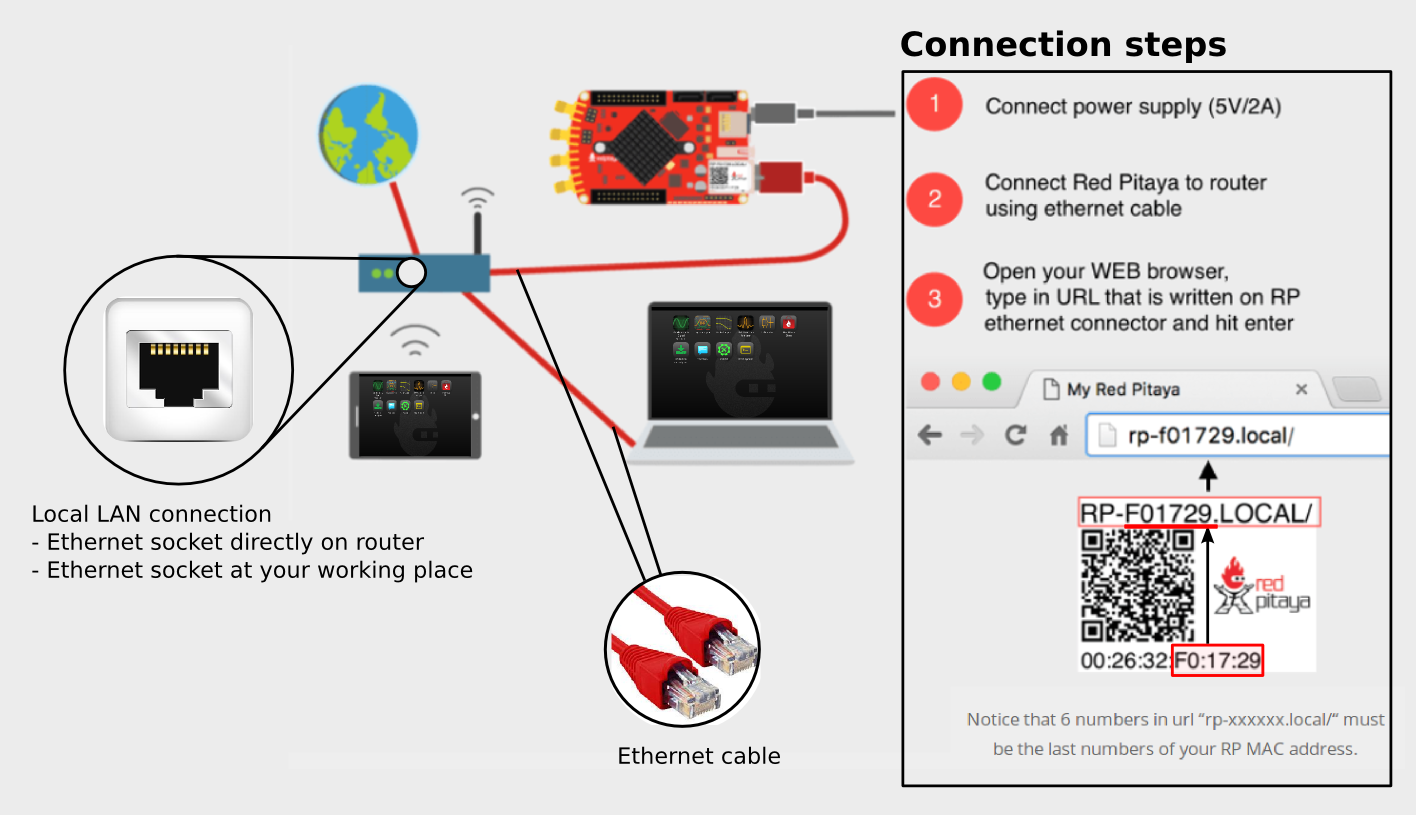
\includegraphics[width=0.9\textwidth]{images2/connect-2} 
		\caption{Connecting your Red Pitaya board to the LAN network.}
		\label{fig:fig1}
	\end{center}
\end{figure}

After the third step you will get a Red Pitaya main page as shown below in Figure \ref{fig:squeme2}.

\begin{figure}[!h]
	\begin{center}
		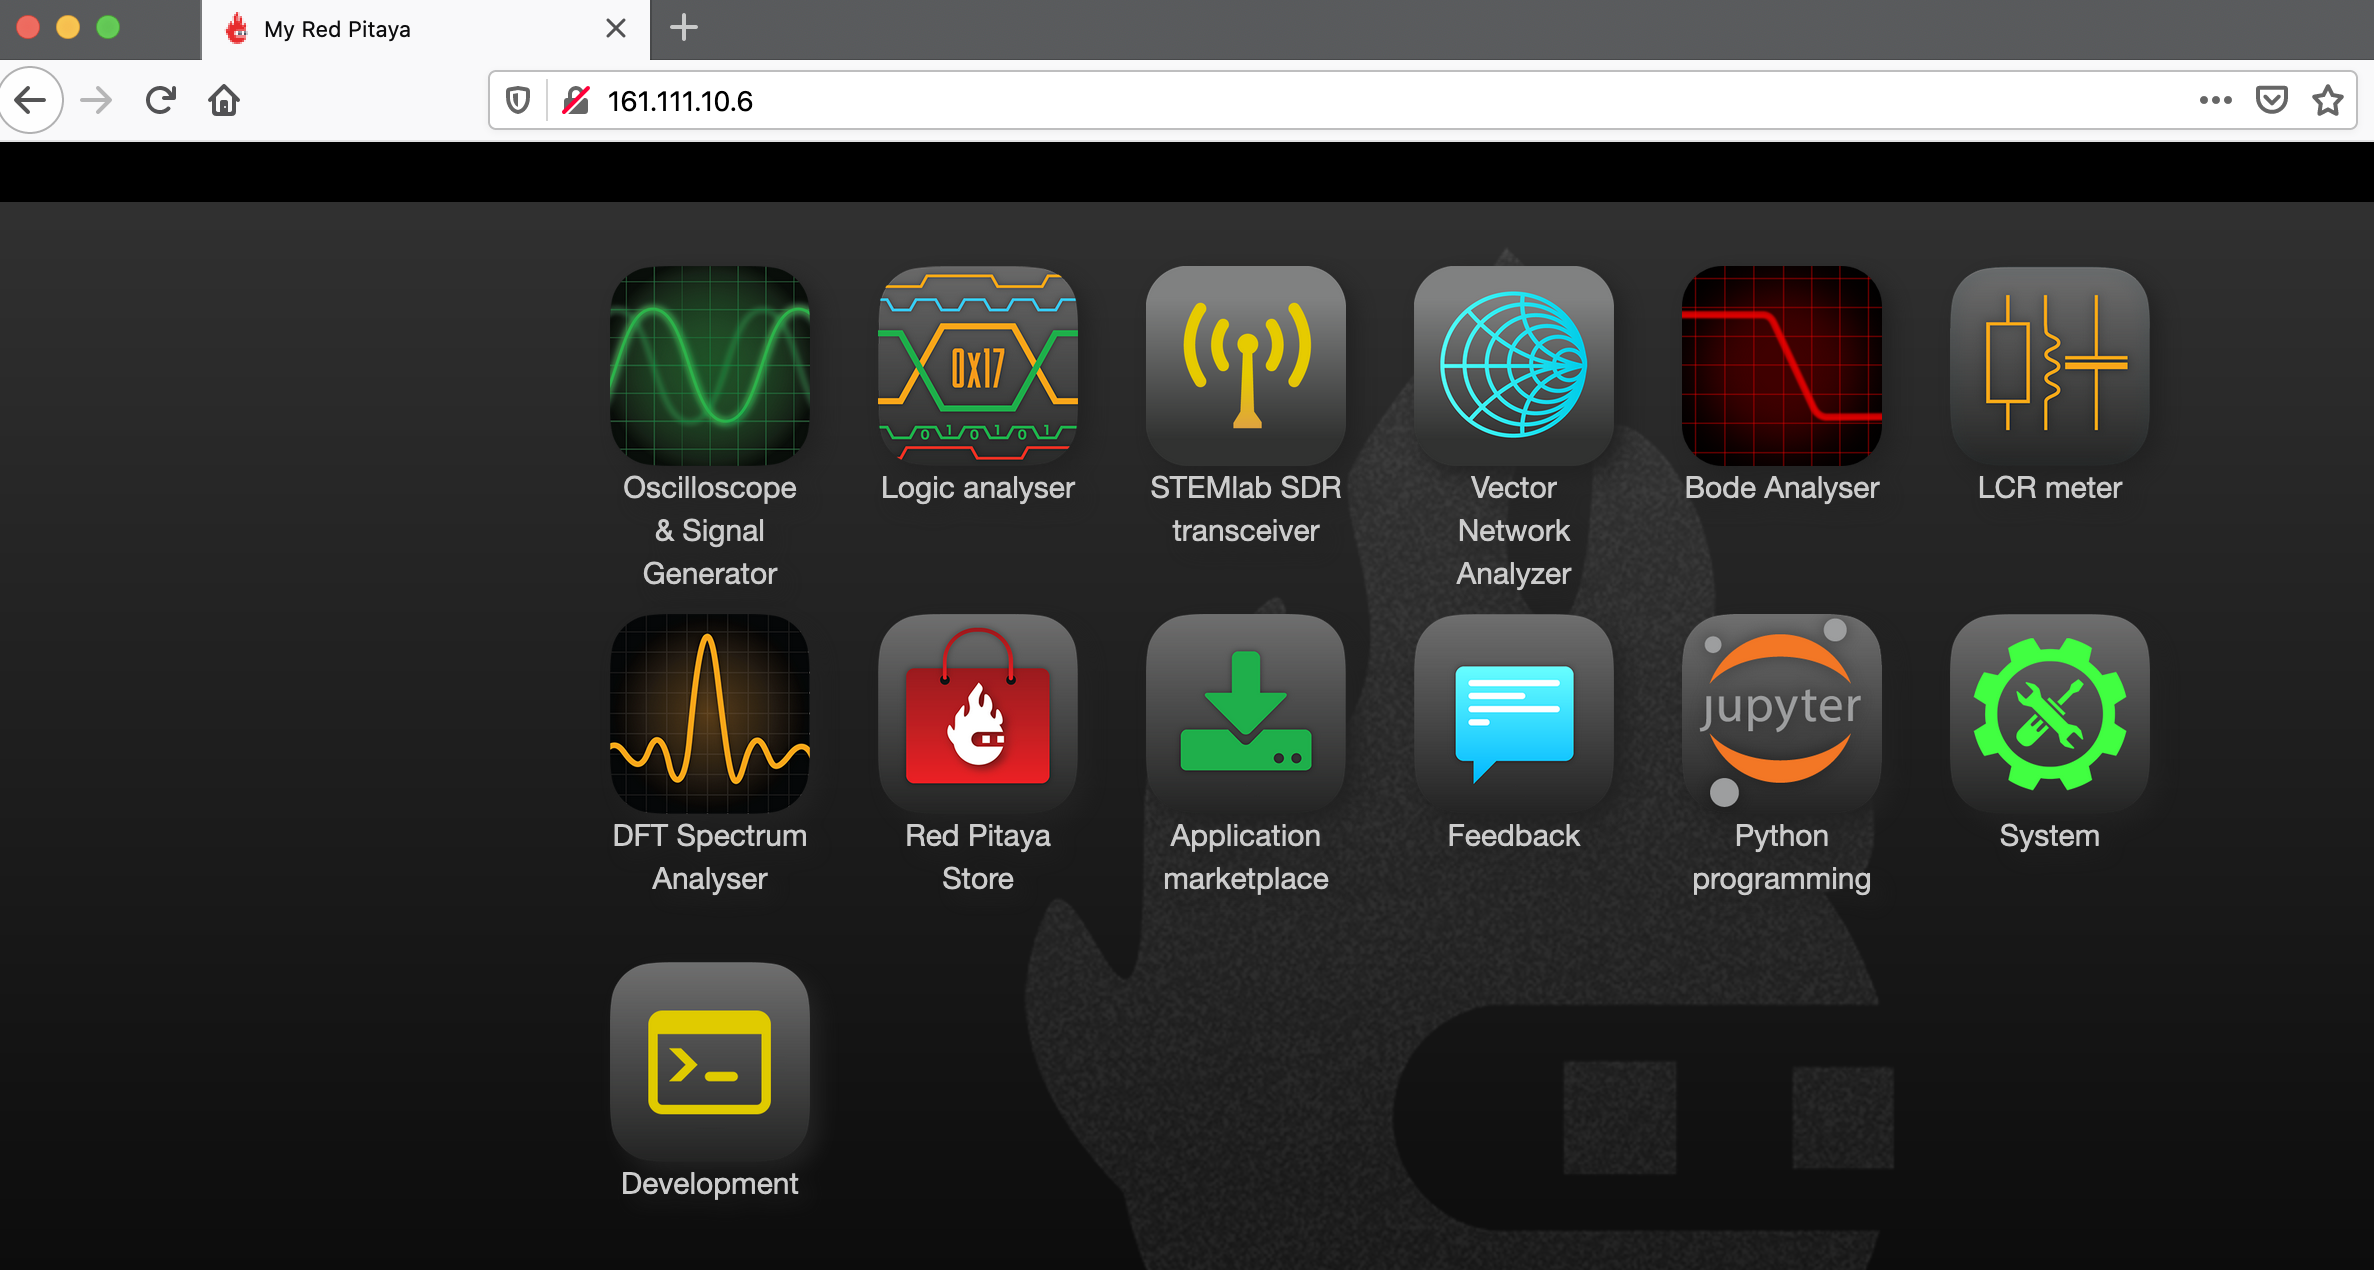
\includegraphics[width=1\textwidth]{images2/connect-3} 
		\caption{Red Pitaya main page user interface.}
		\label{fig:squeme2}
	\end{center}
\end{figure}

\item Direct ethernet cable connection: It requires additional setting on users PC and Red Pitaya board. If there are some restrictions for the user to have Red Pitaya board on the DHCP LAN network permanently, there is a possibility to directly connect to the Red Pitaya board. We have used this configuration for the setup and the measurements. Direct ethernet connection is enabled and some additional settings on the user’s PC (static IP configuration) are necessary in order to set connection correctly. The only step needed is to plug the ethernet cable from your PC to the Red Pitaya board (see Figure \ref{fig:squeme}).

\begin{figure}[!h]
	\begin{center}
		\includegraphics[width=0.7\textwidth]{images2/connect-0} 
		\caption{Red Pitaya and PC direct connection.}
		\label{fig:squeme}
	\end{center}
\end{figure}

a) Connect the ethernet cable and wait 30 sec. 

b) Open the web browser and type rp-xxxxxx.local/ in the URL field.

\item Static IP configuration: This type of connection requires additional settings\footnote{This connection is also arranged via Network manager application so users should first have access to the LAN (DHCP) network in order to arrange static IP on the Red Pitaya board.}

\begin{figure}[!tp]
	\begin{center}
		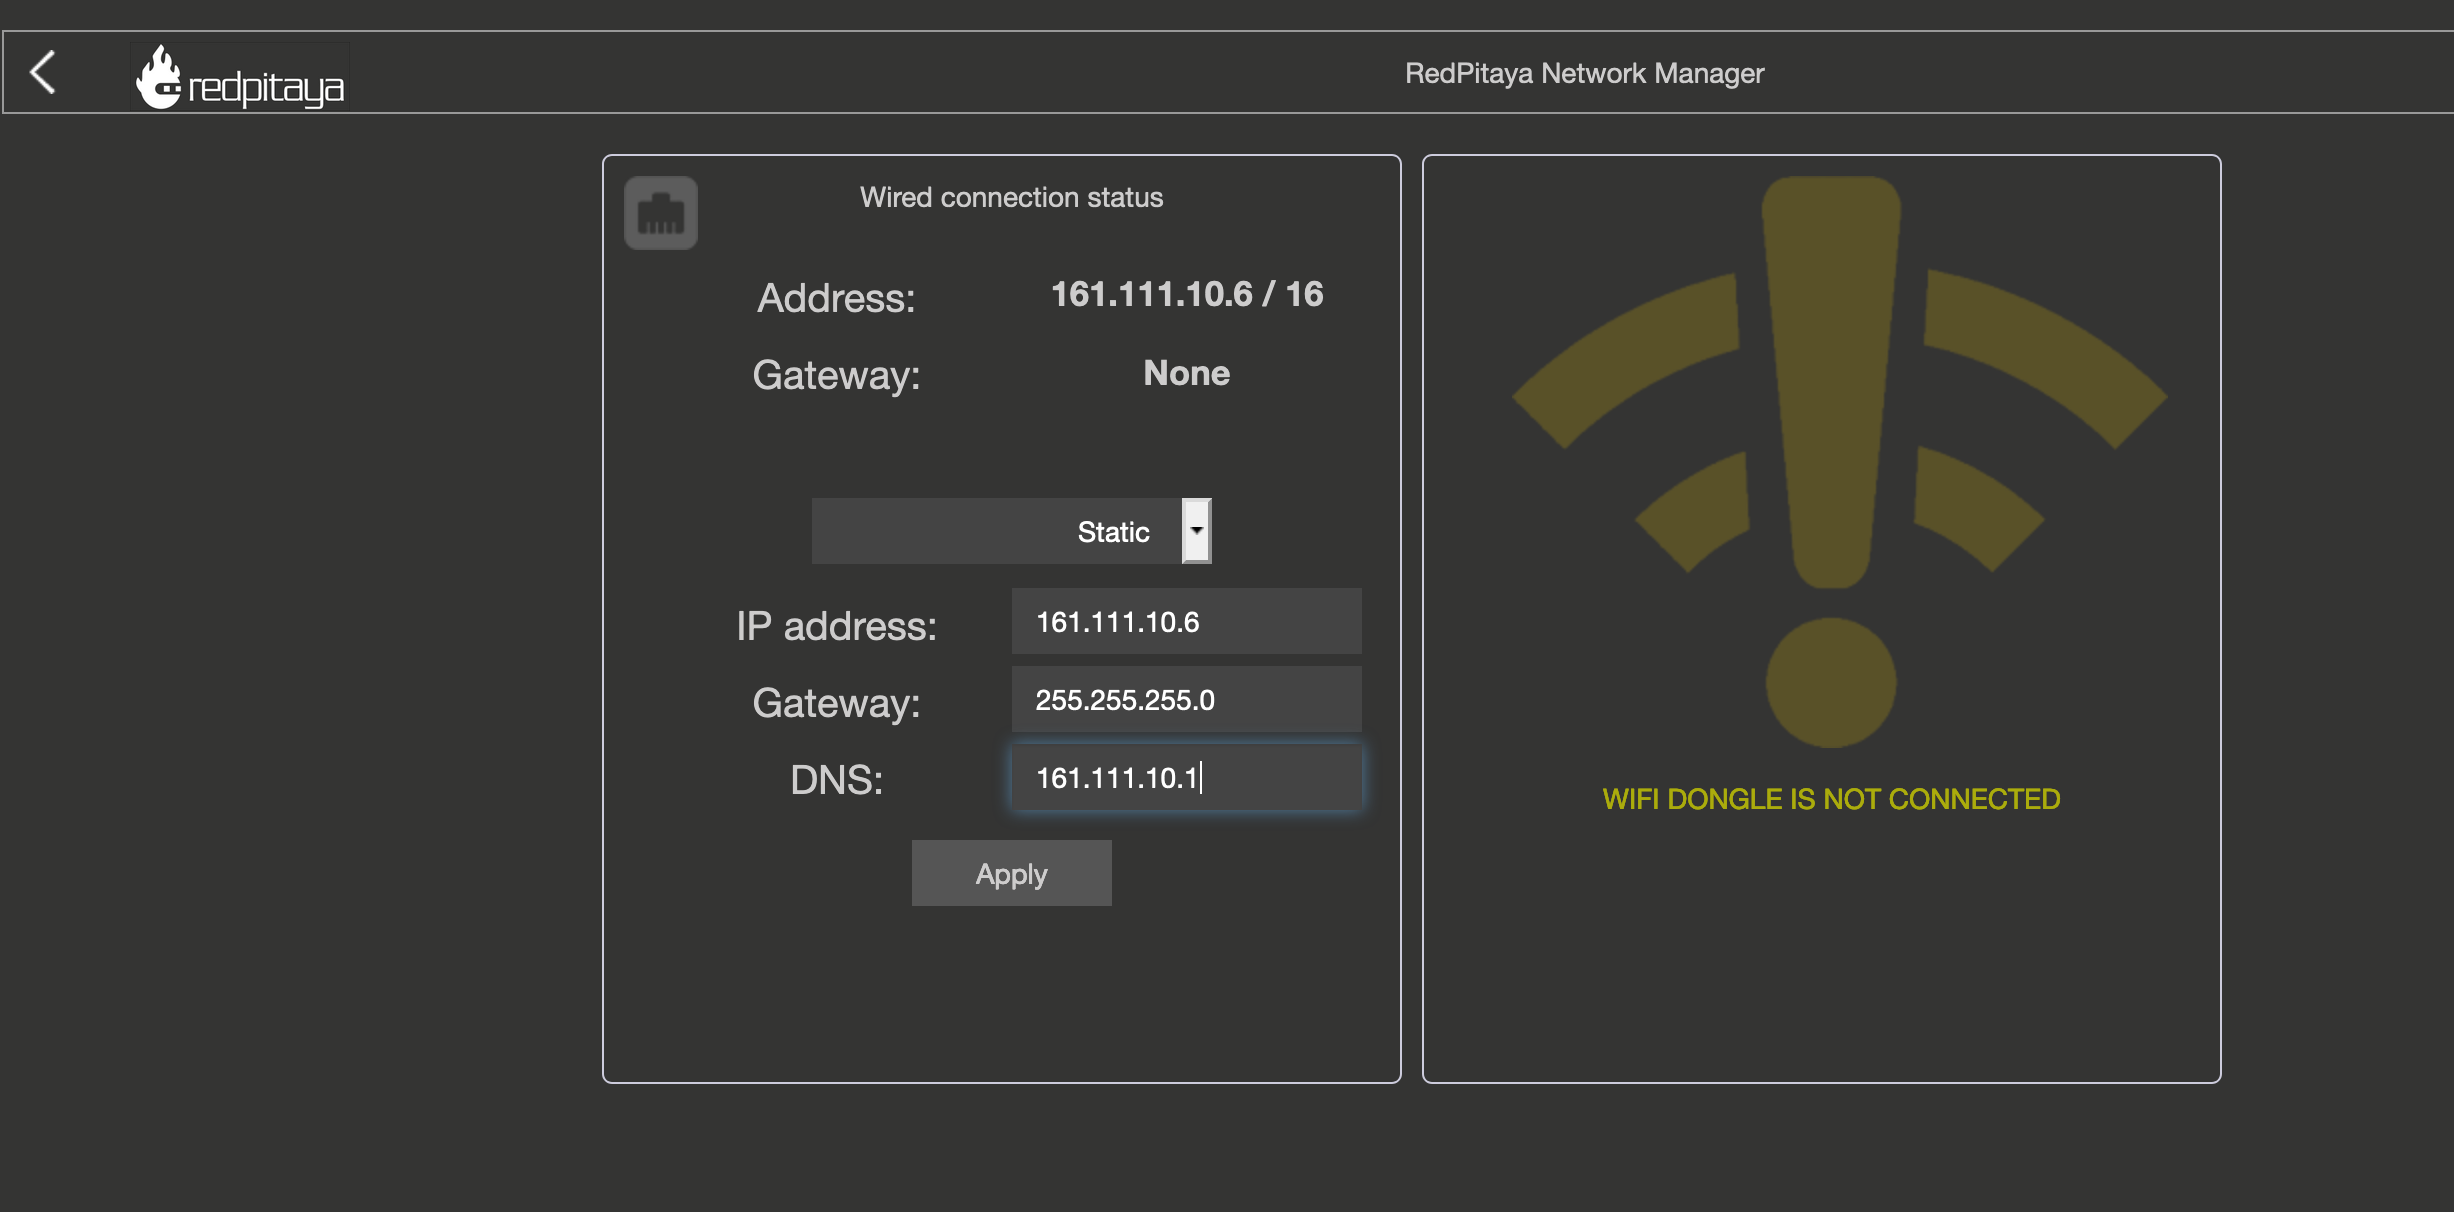
\includegraphics[width=1\textwidth]{images2/connect-11} 
		\caption{Red Pitaya IP configuration.}
		\label{fig:ip}
	\end{center}
\end{figure}

a) First step in connecting Red Pitaya board directly to LAN network and setting a static IP on it. Once you are successfully connected to your Red Pitaya board, open the network manager and chose static option (i.e. IP 161.111.10.5, Gateway 255.255.255.0, DNS: 161.111.10.1). Input the static IP and click Apply (see Figure \ref{fig:ip}).

b) Second step is to set a network setting on the PC\footnote{Once you have this settings arranged, connect Ethernet cable between your Red Pitaya board and PC, open web browser, in the web browser URL field input chosen Red Pitaya board static IP (in our example 161.111.10.6) and press enter}:

- Select manual method. Press Add button and insert static IP address of your PC (must be different from the IP address of the Red Pitaya board). Netmask (input: 255.255.255.0). Getaway (can be left empty). DNS servers (can be left empty) and click Save button.

- We can check the IP configuration from our PC by using the terminal. Writing the ``arp -a" command, the terminal shows the IP address and the ethernet boards that are connected to the LAN. Figure \ref{fig:connect} shows our particular configuration: 

\end{itemize}

\begin{figure}[!h]
	\begin{center}
		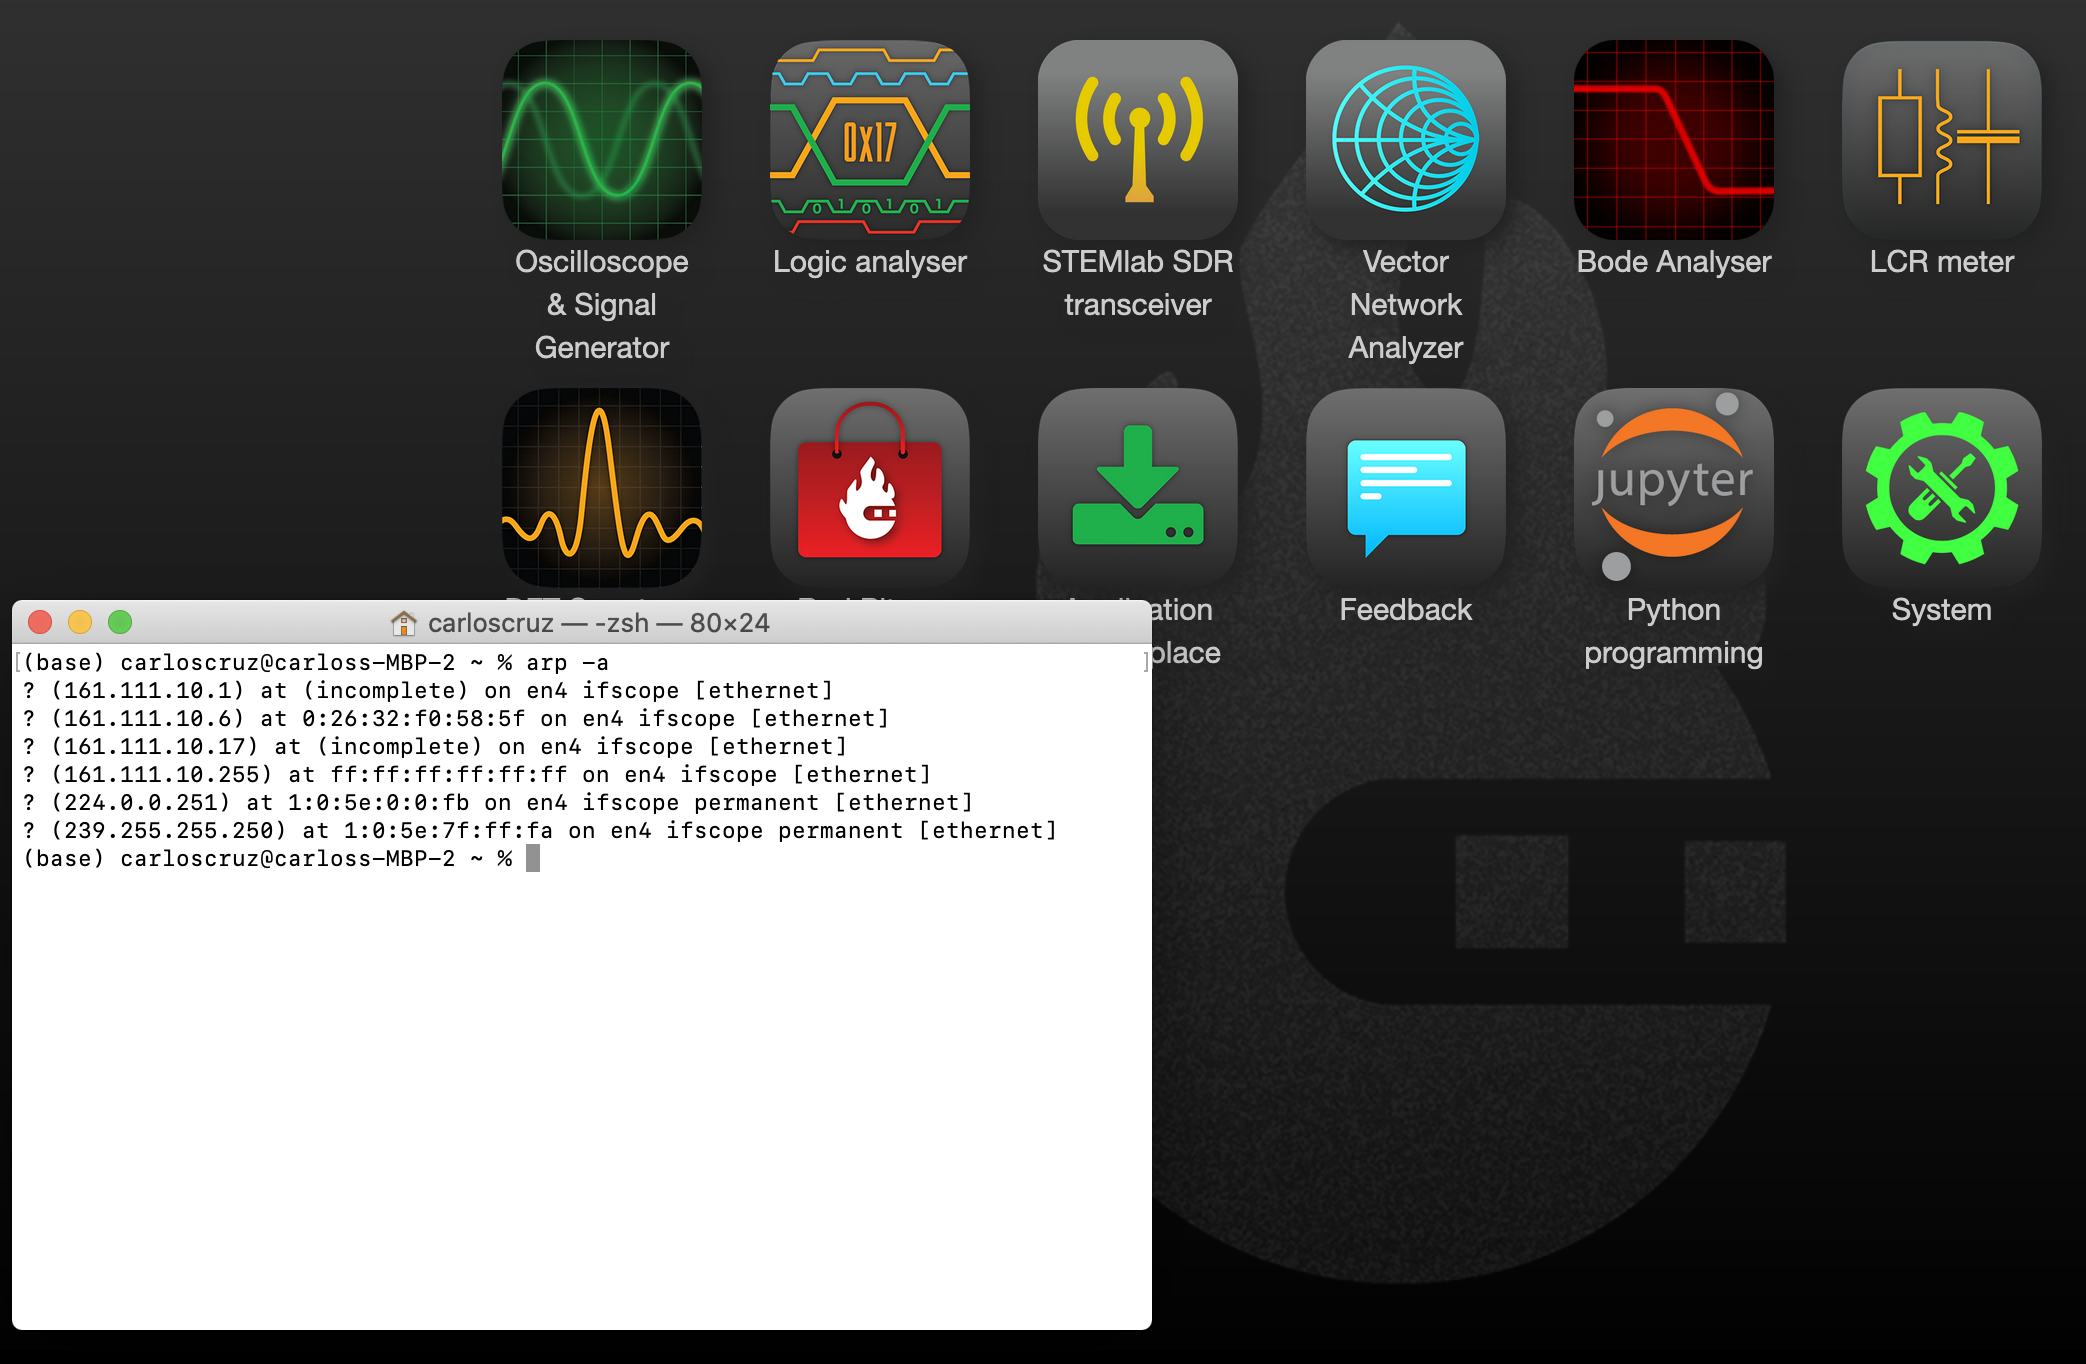
\includegraphics[width=1\textwidth]{images2/connect-check} 
		\caption{Connection board status and Red Pitaya interface.}
		\label{fig:connect}
	\end{center}
\end{figure}


%\begin{figure}[!h]
%	\begin{center}
%		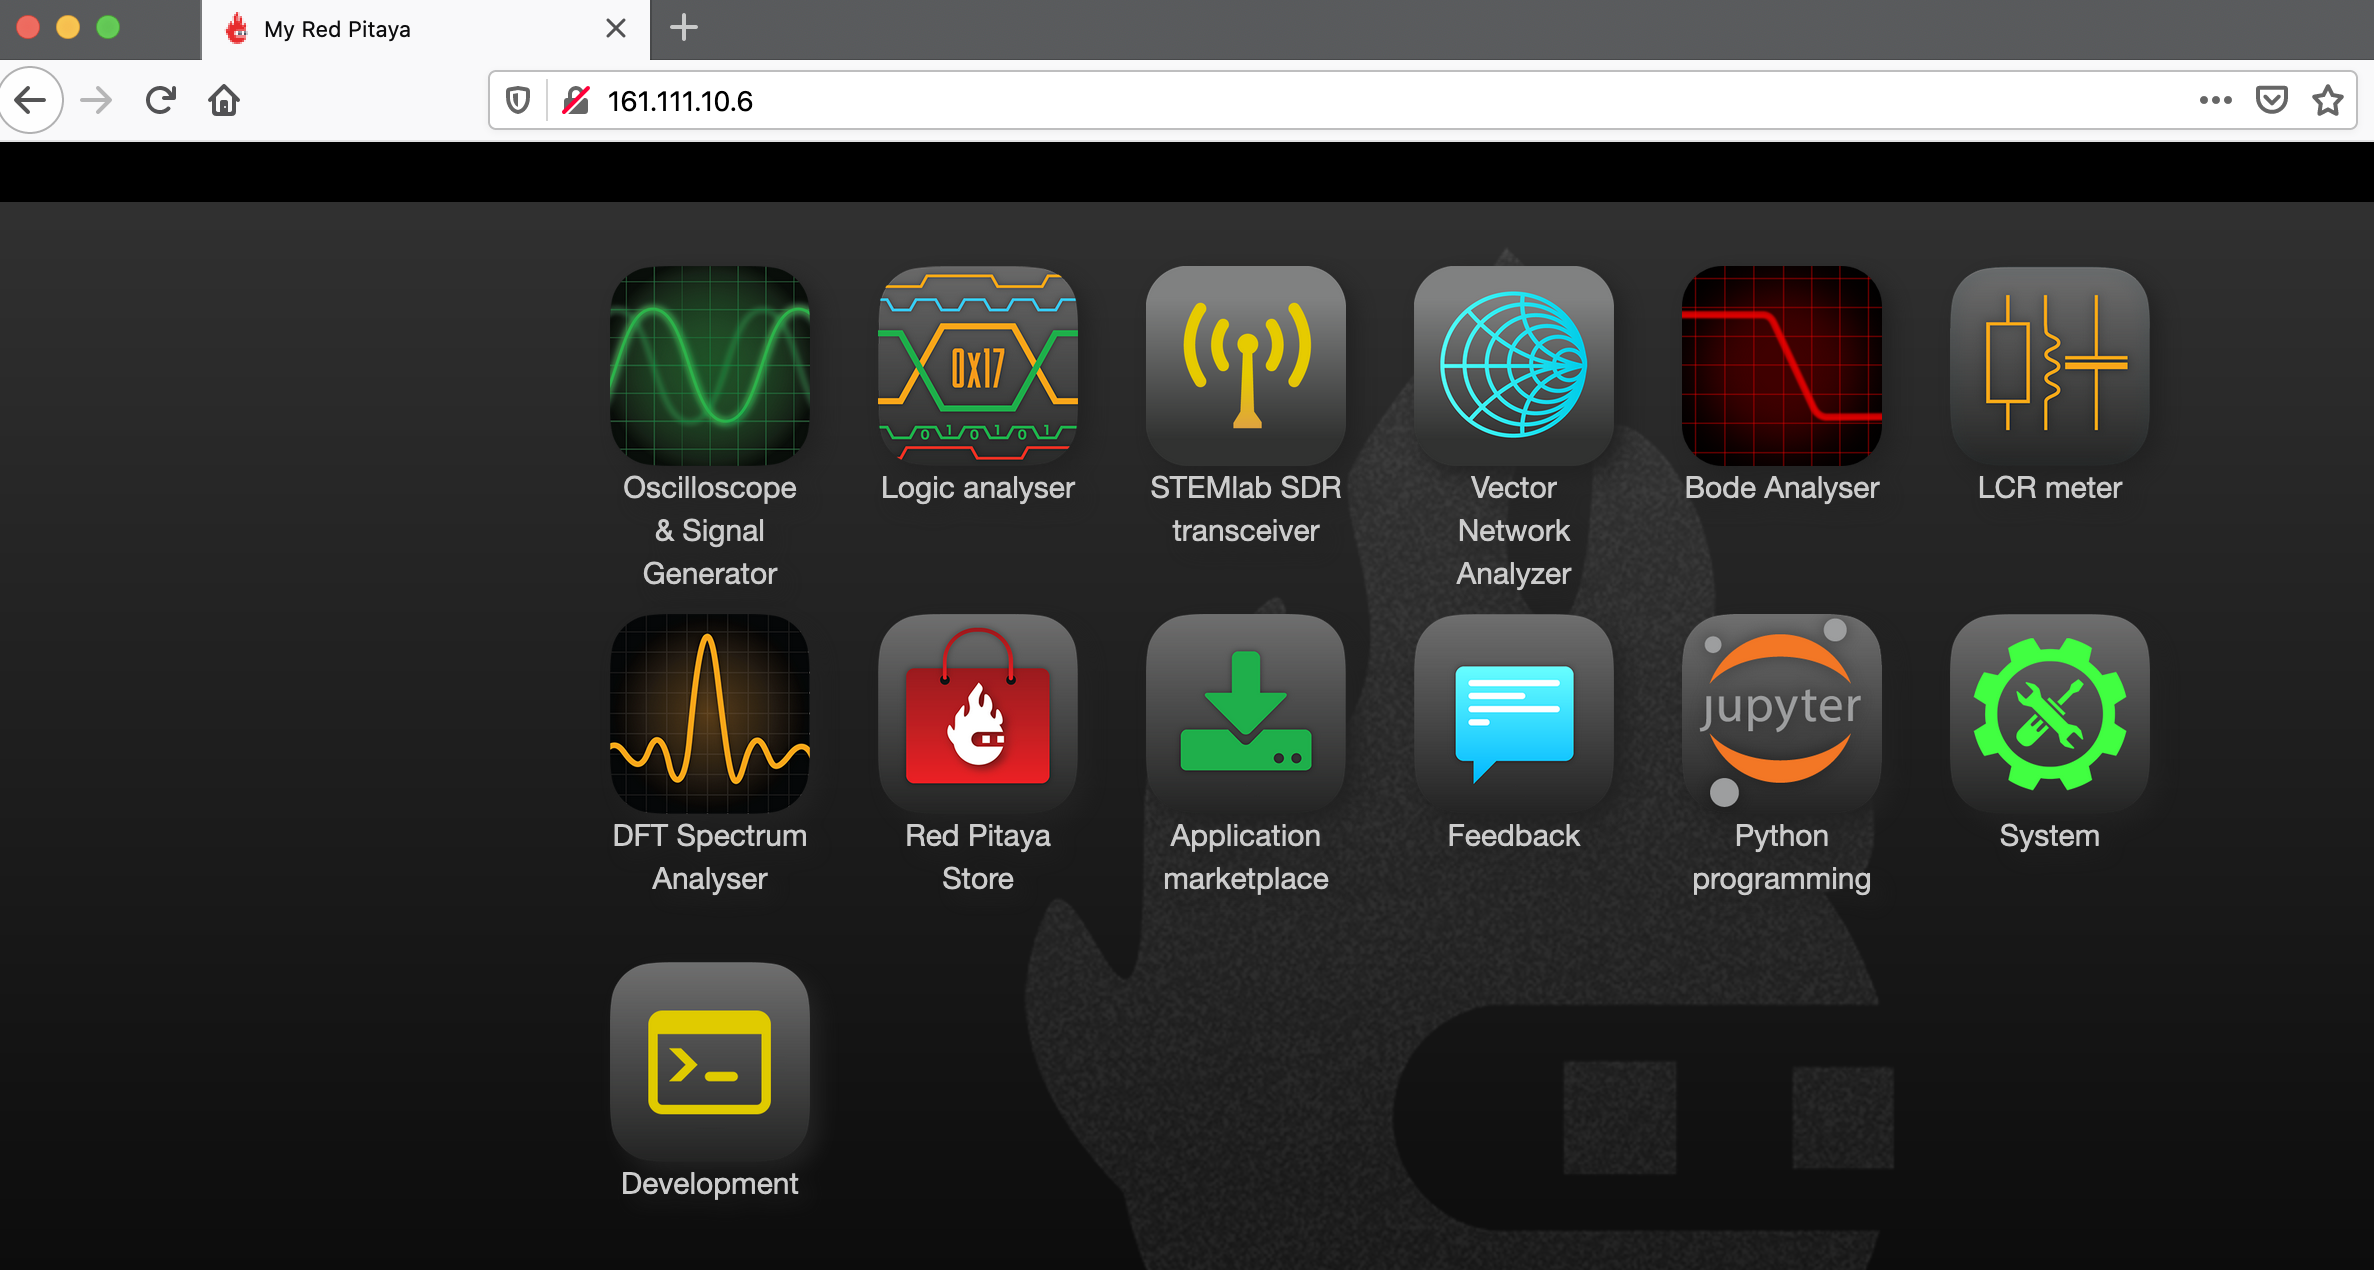
\includegraphics[width=0.7\textwidth]{images2/connect-3} 
%		\caption{Setup.}
%		\label{fig:setup}
%	\end{center}
%\end{figure}


%Once you have this settings arranged, connect Ethernet cable between your Red Pitaya board and PC, open web browser, in the web browser URL field input chosen Red Pitaya board static IP (in our example 161.111.10.6) and press enter.

\section{Red Pitaya as oscilloscope and signal generator}

The connectors ``IN1" and ``IN2" are the fast inputs on the Red Pitaya board and are used to measure high frequency signals. Both channels can be adjusted separately. Each input on the board is associated with two jumpers. These jumpers have the expected input voltage at the respective channel preselected. The jumper must be set in pairs for each input. 

LV: ± 1V (Low Voltage /the  signal level is in the range -1…+1V)

HV :HV: ± 20V (High Voltage /the  signal level is in the range -20…+ 20V)

The real highlight of Red Pitaya’s oscilloscope is the signal generator. It can be used for various types of periodic signals with a maximum amplitude of ± 1V (2V P2P) produced, and ``OUT1" and ``OUT2" connectors. The maximum frequency that can be output is largely dependent on the signal form. For instance, Figure \ref{fig:signal} shows the generated sinusoidal signal that we have generated for our measurements (in blue) and the measured signal at the input IN1(in yellow).

\begin{figure}[!h]
	\begin{center}
		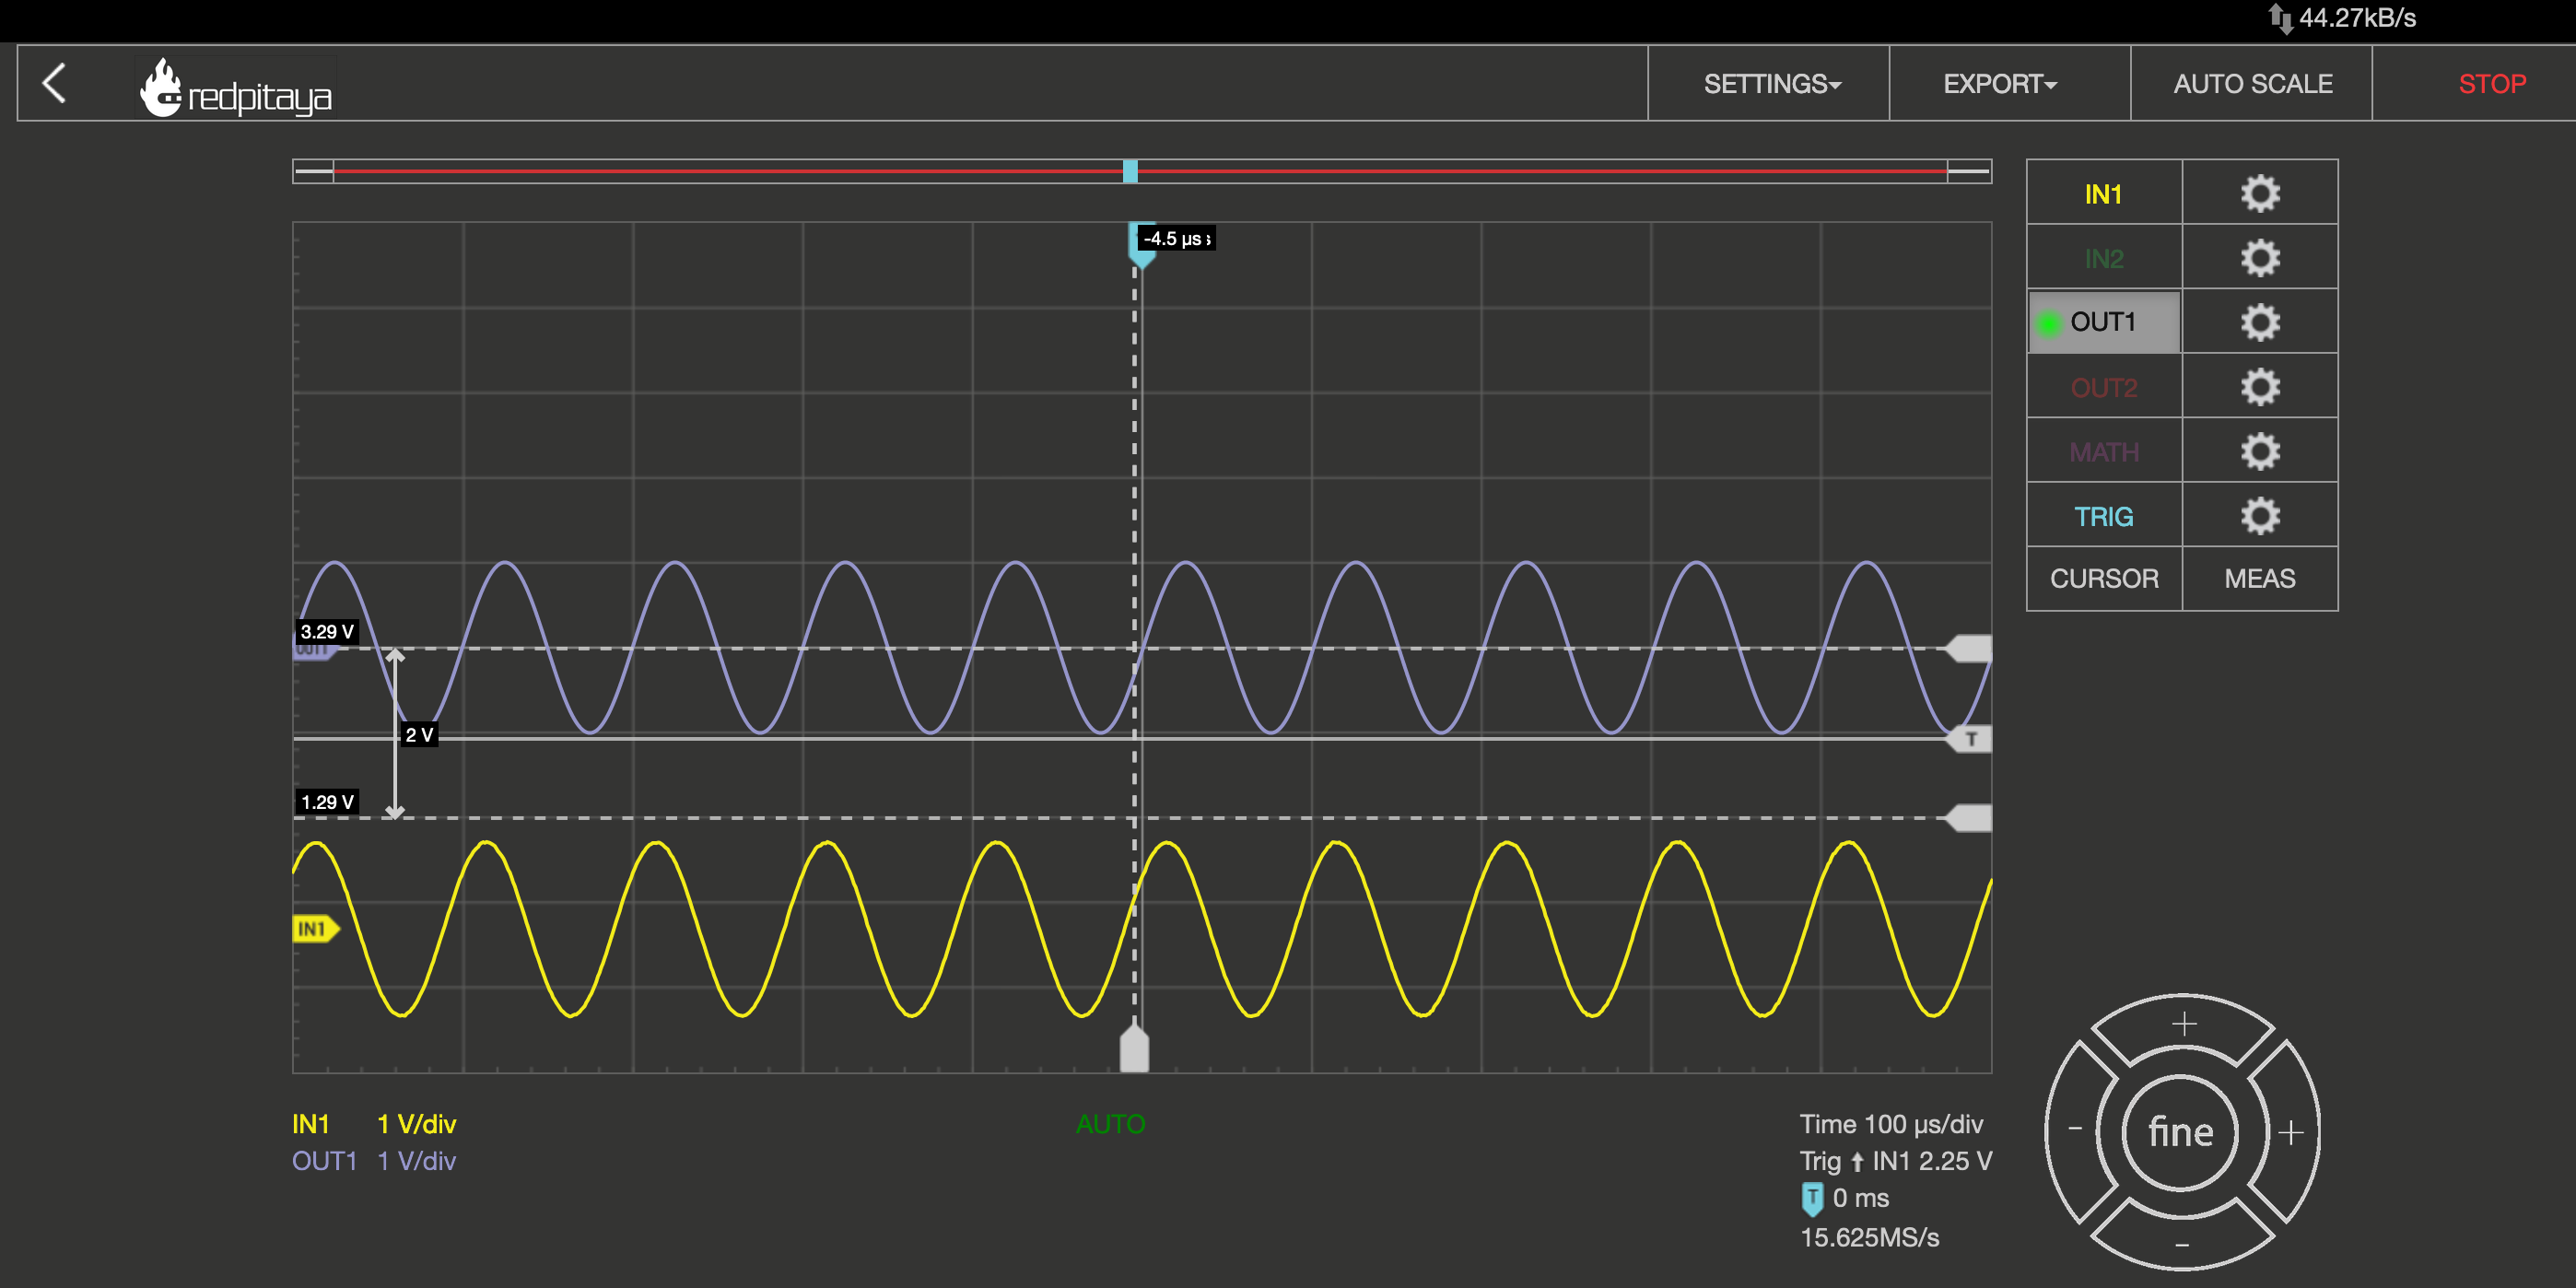
\includegraphics[width=1\textwidth]{images2/connect-14} 
		\caption{Generated signal by the Red Pitaya board.}
		\label{fig:signal}
	\end{center}
\end{figure}

\section{Server SCPI Configuration}

The Standard Commands for Programmable Instrumentation (SCPI) interface/environment is commonly used to control instruments for development, research or test automation purposes. SCPI uses a set of SCPI commands that are recognized by the instruments to enable specific actions to be taken (e.g. acquiring data from fast analog inputs, generating signals and controlling other periphery of the Red Pitaya STEMLab platform). In order to perform measurements by using LabVIEW software, we need to enable remote control of Red Pitaya board. SCPI configuration needs to be activated as we need to run SCPI server application (see Figure \ref{fig:squemeXX}).

\begin{figure}[!h]
	\begin{center}
		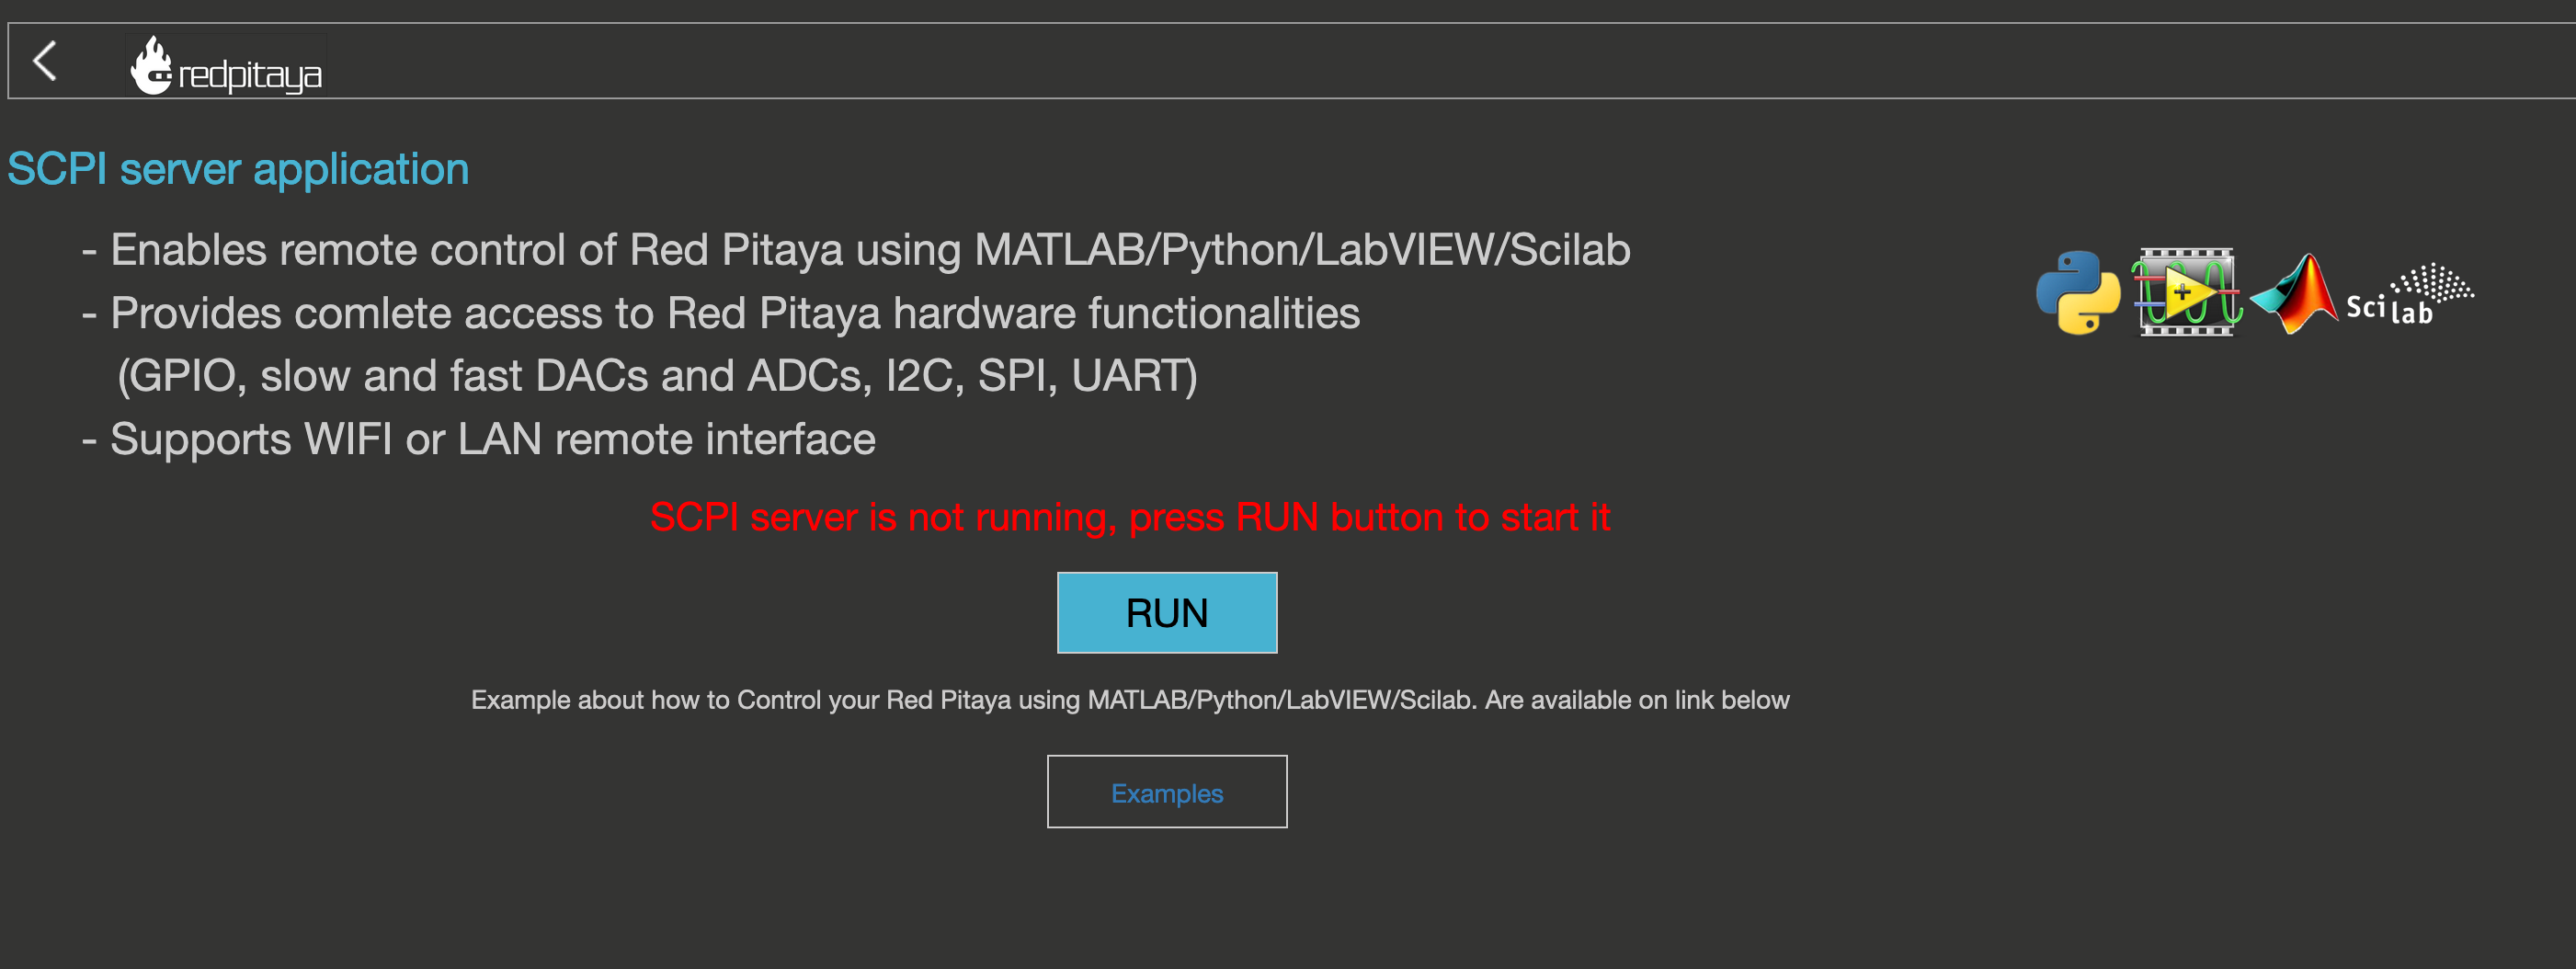
\includegraphics[width=1\textwidth]{images2/connect-12} 
		\caption{Red Pitaya SCPI setup configuration.}
		\label{fig:squemeXX}
	\end{center}
\end{figure}

Once SCPI server is running (see Figure\ref{fig:squemexxx}), webbrowser needs to be closed.

\begin{figure}[!h]
	\begin{center}
		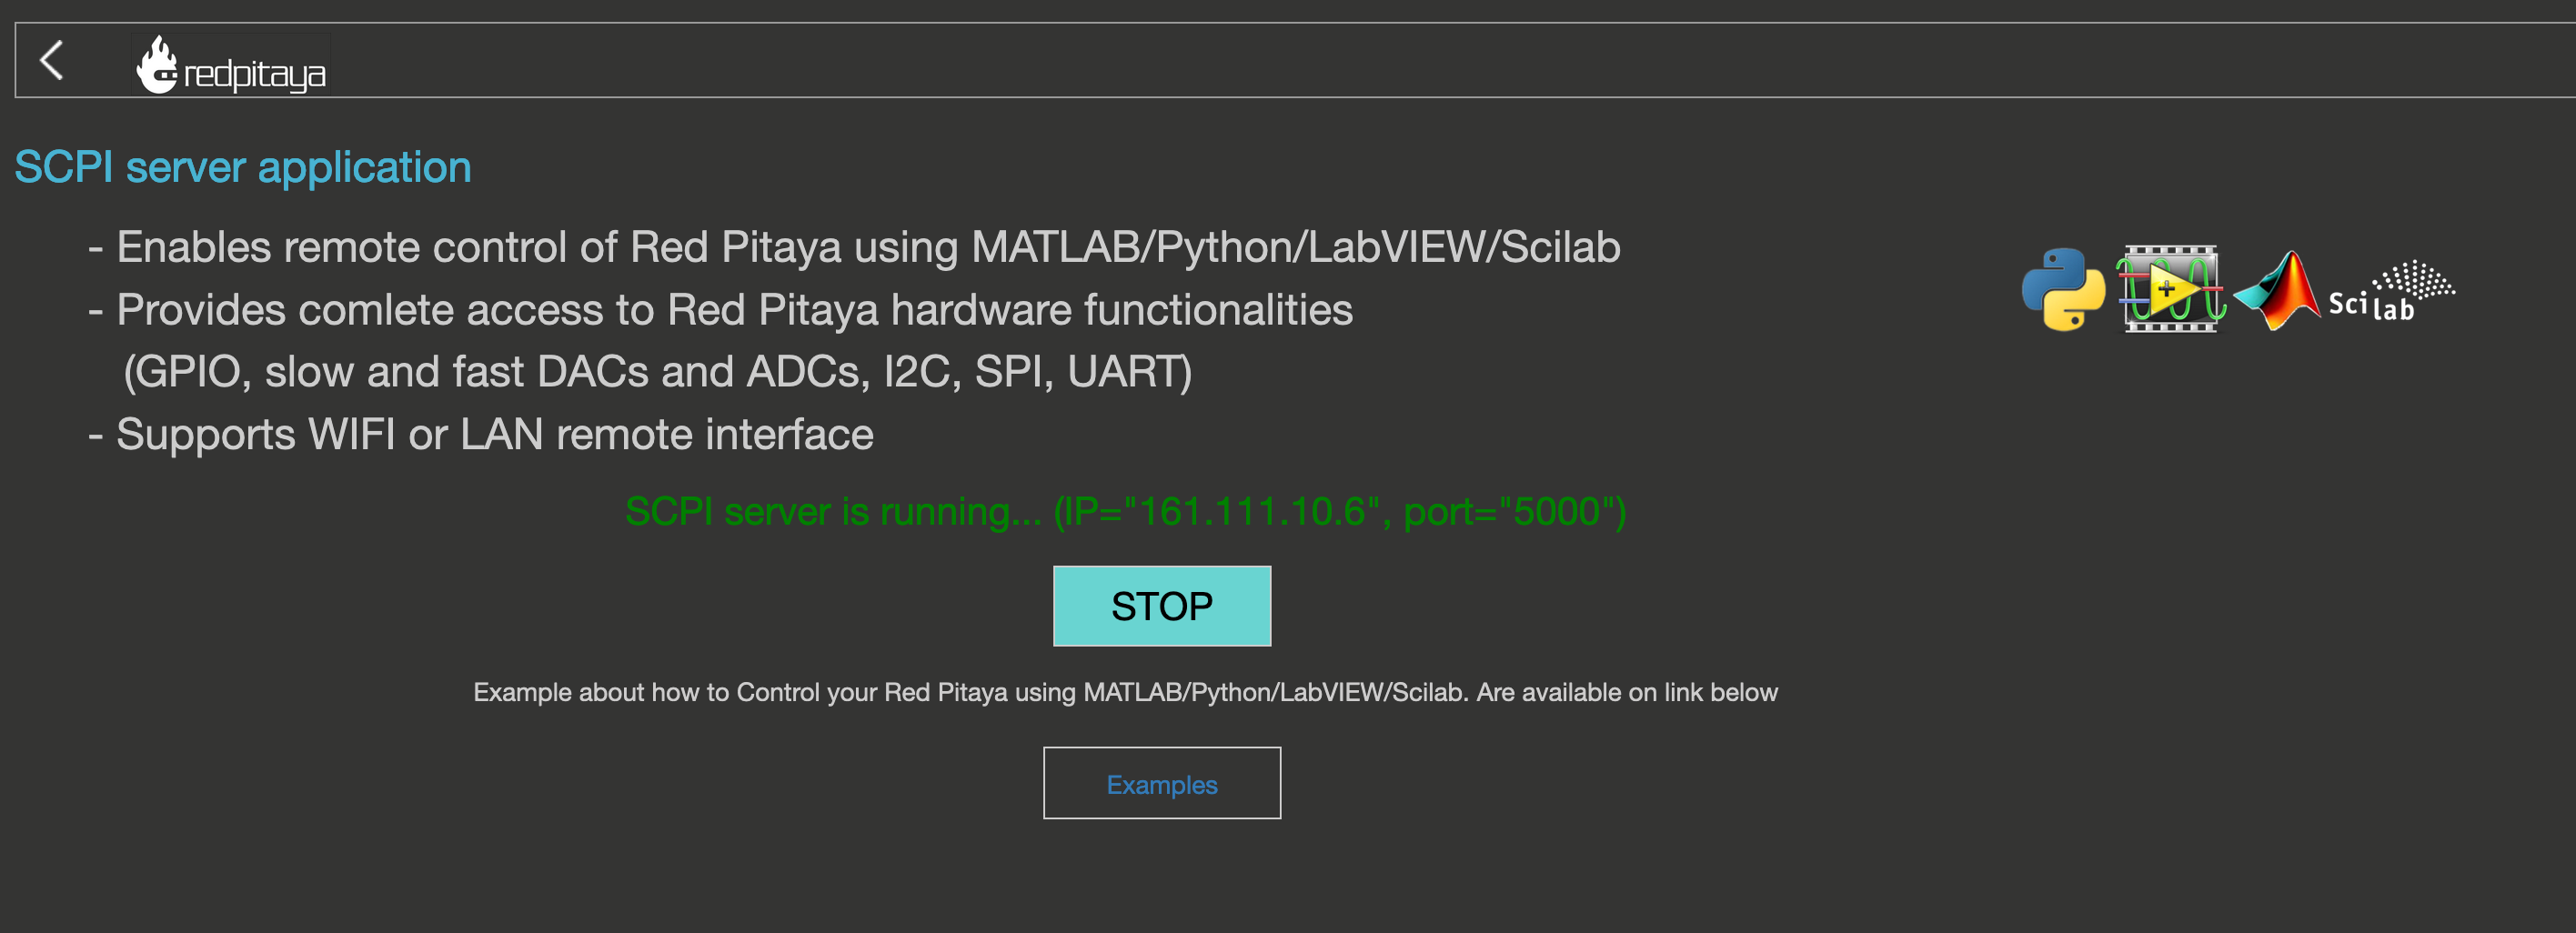
\includegraphics[width=1\textwidth]{images2/connect-13} 
		\caption{Red Pitaya SCPI server status.}
		\label{fig:squemexxx}
	\end{center}
\end{figure}


\begin{figure}%[!h]
	\begin{center}
		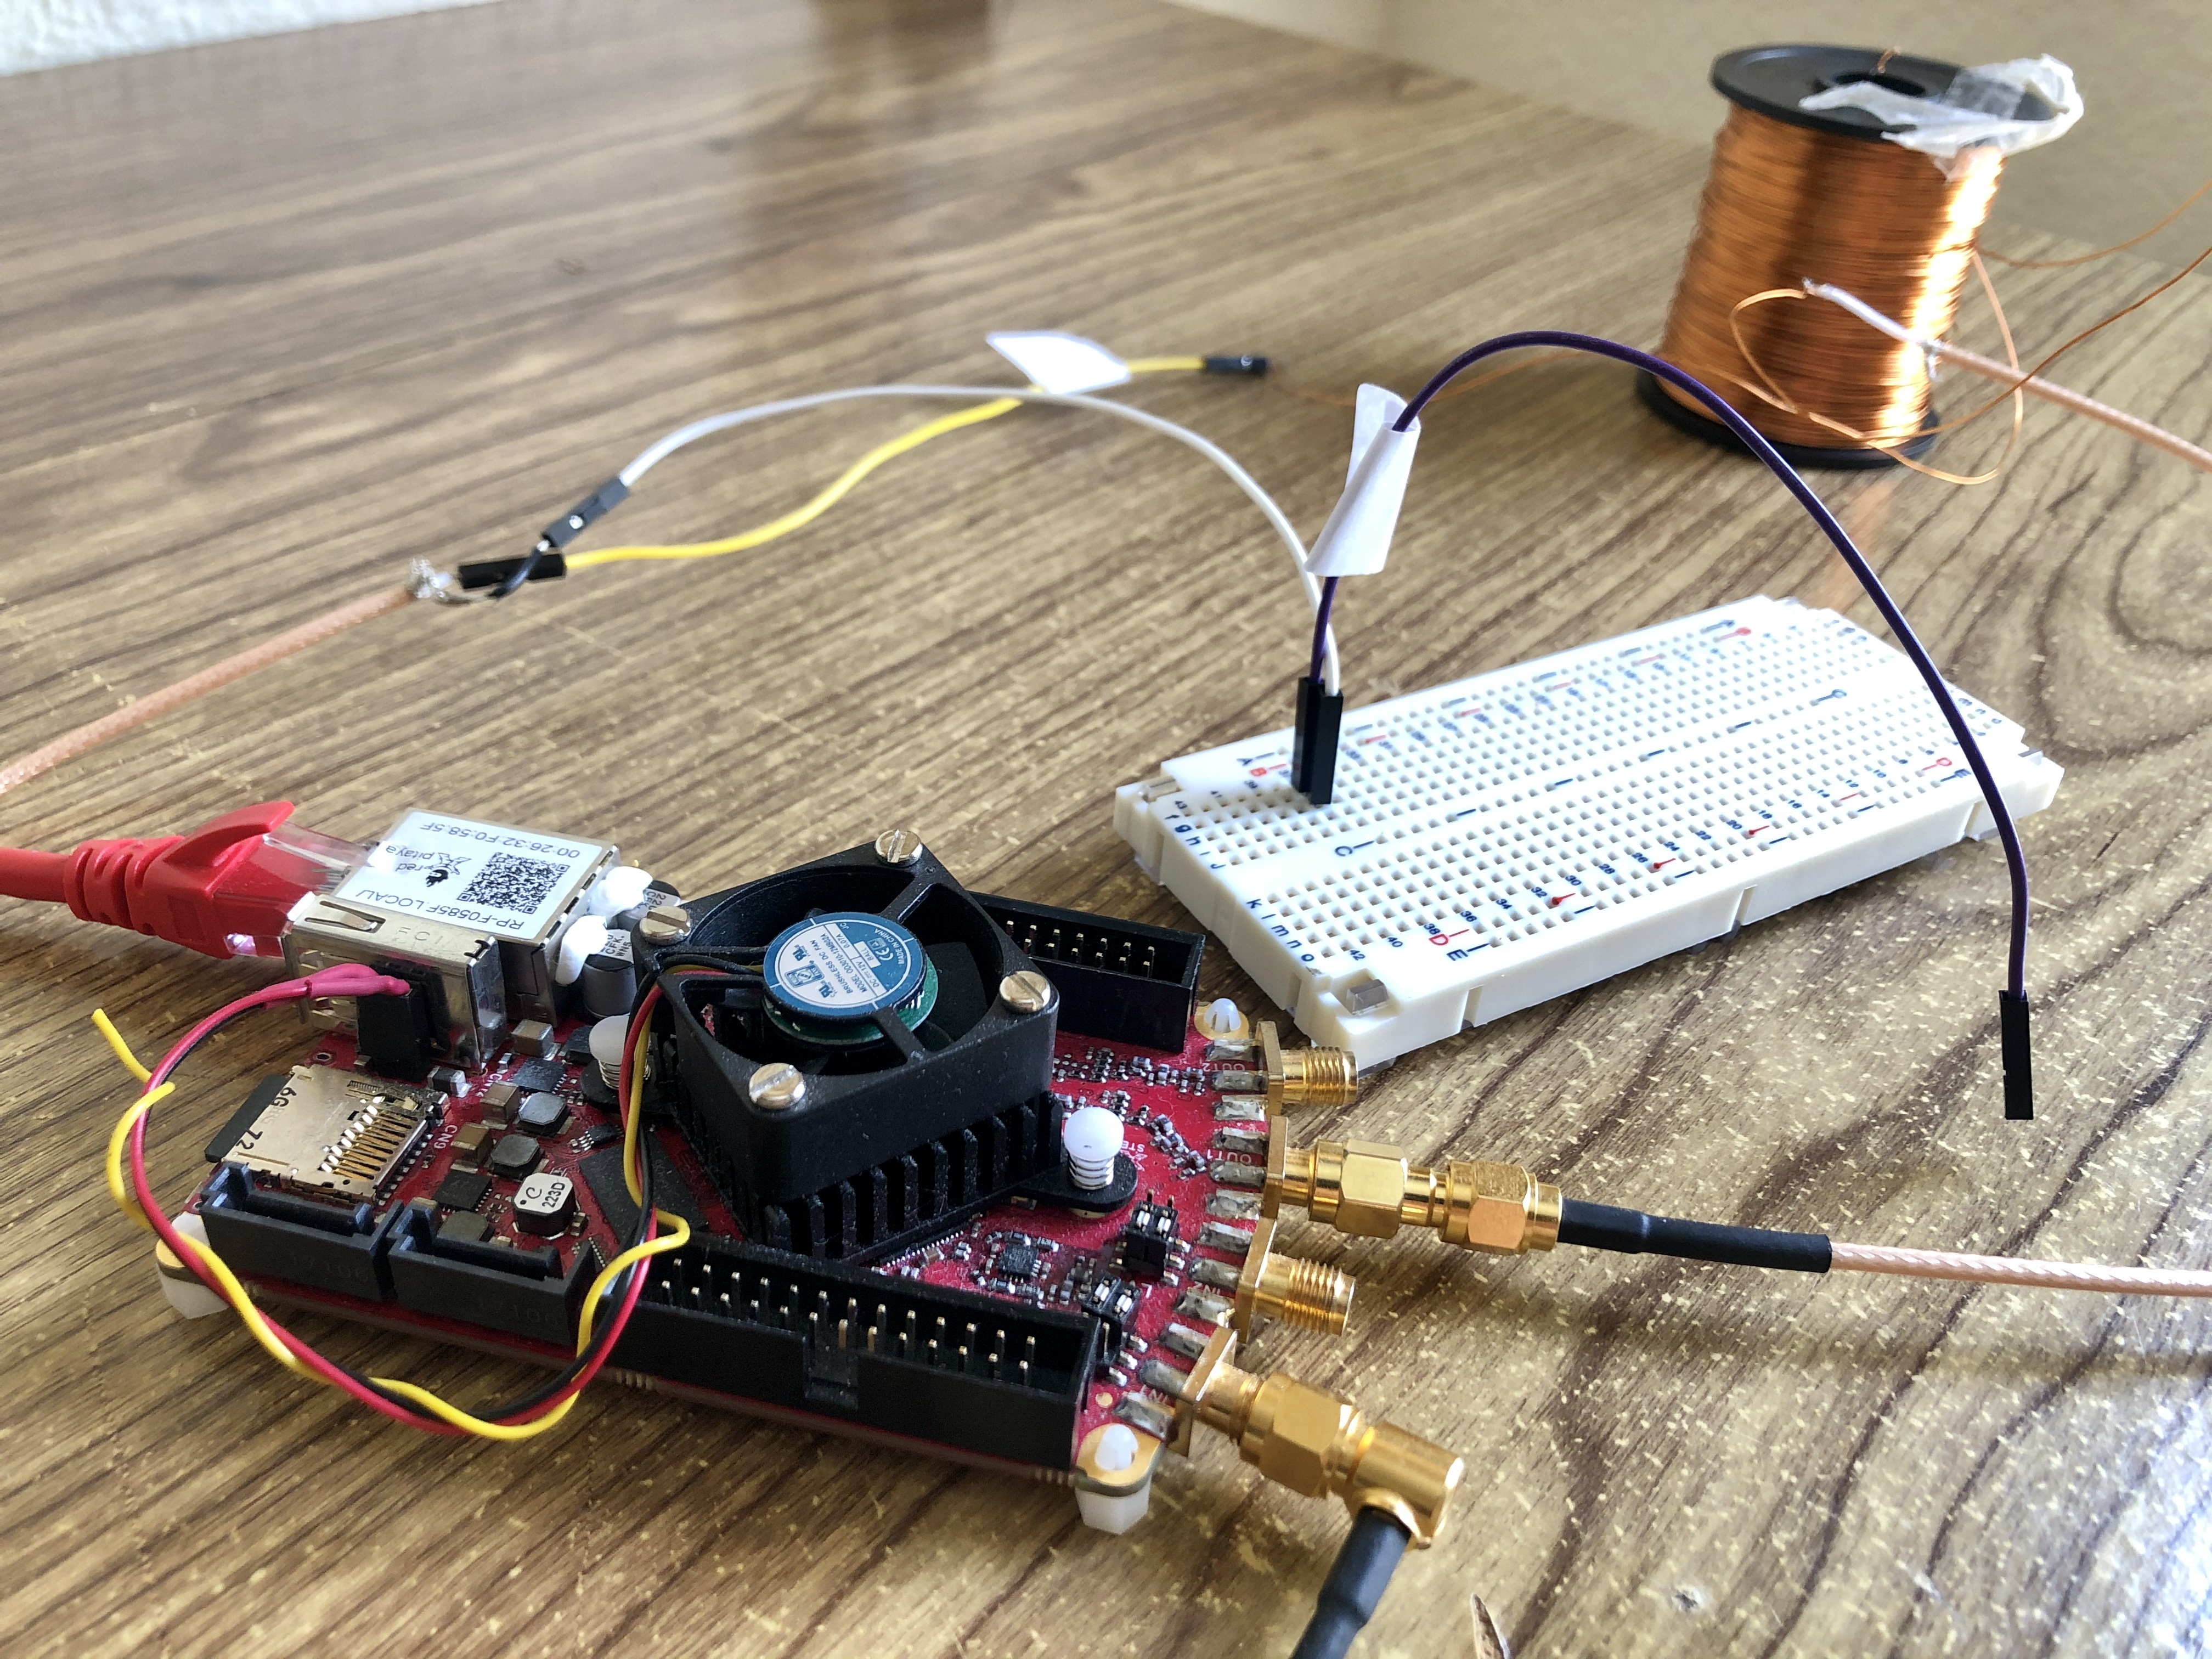
\includegraphics[width=0.6\textwidth]{images2/setup.png} 
		\caption{Experimental setup.}
		\label{fig:setup}
	\end{center}
\end{figure}




\section{Software}

The Figure \ref{fig:setup} shows the setup configuration for the measurements. It is composed by the Red Pitaya \cite{redpitaya}, which is connected to the copper coil  at one end. The other end of the copper coil is connected to the Red Pitaya input. The ground is connected by the protoboard. We generate a sinusoidal signal (58KHz) that is measured from the copper coil (blue). 

\begin{figure}[!h]
	\begin{center}
		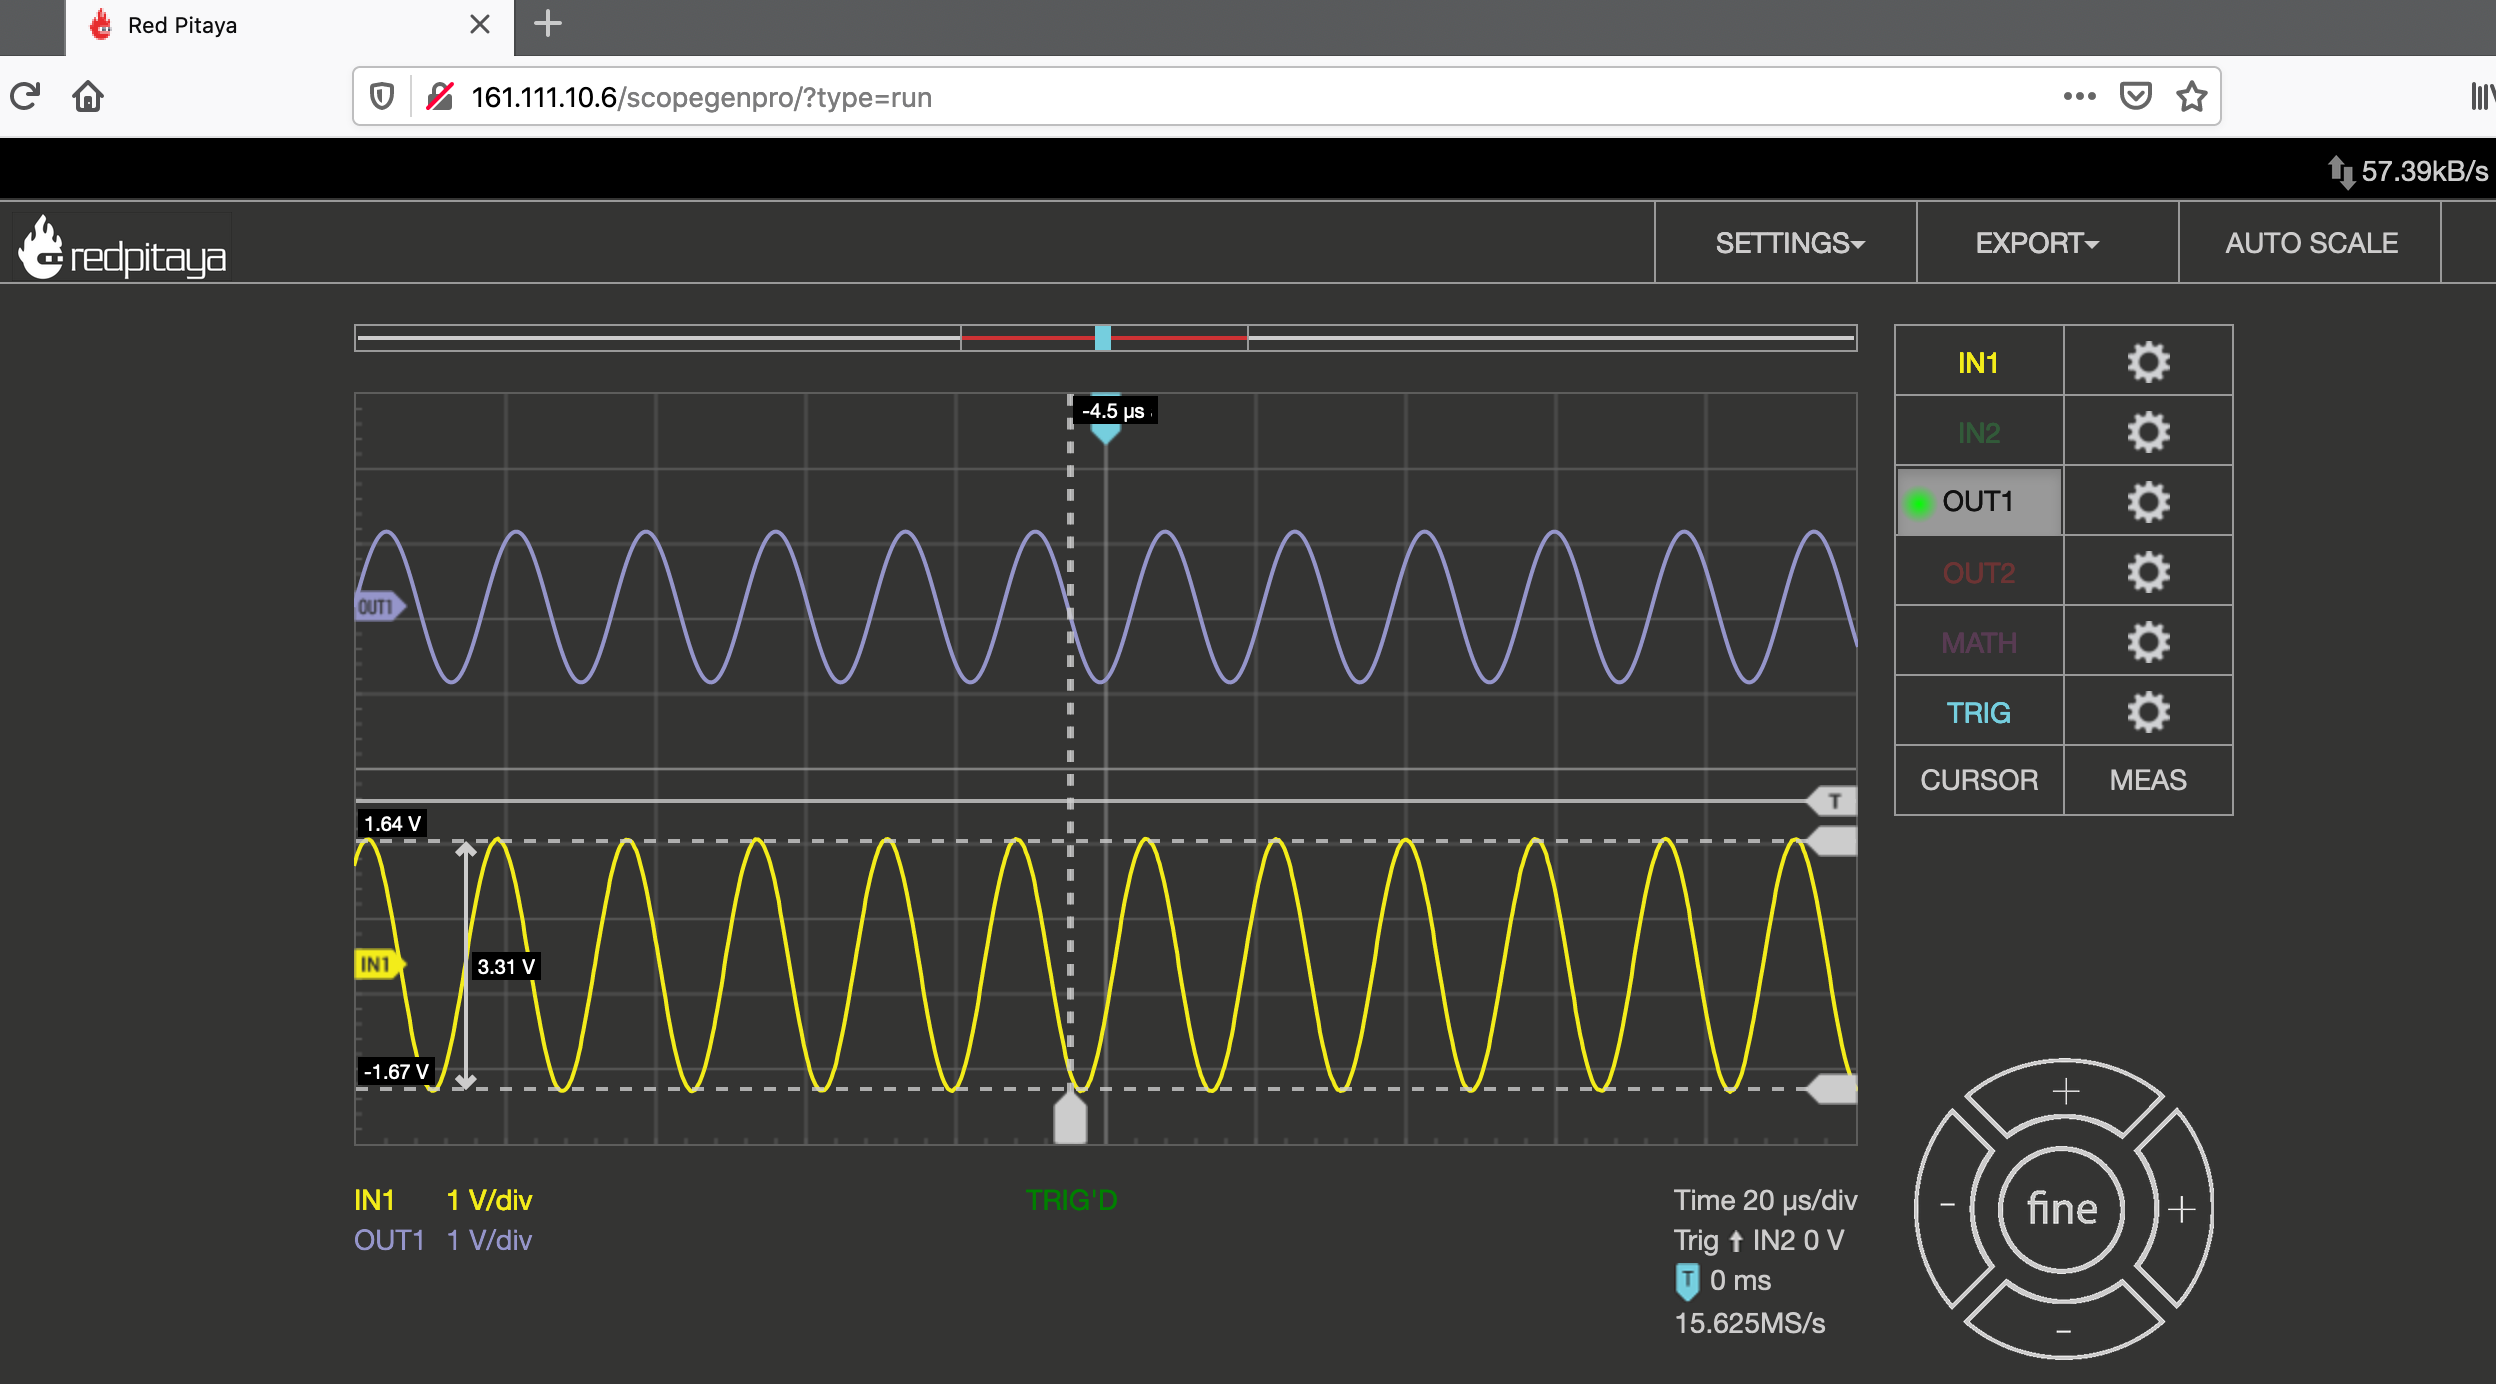
\includegraphics[width=0.8\textwidth]{images2/measurement1} 
		\caption{Sinusoidal generated signal (blue) and reference signal (yellow).}
		\label{fig:m1}
	\end{center}
\end{figure}

The Figure \ref{fig:m1} presents an amplitude value of  3.31V (yellow) and it is asigned as reference value. The measurement present a variation in amplitude of 2.67V when the system measures the magnetic field (see Figure \ref{fig:m2}).

\begin{figure}[!h]
	\begin{center}
		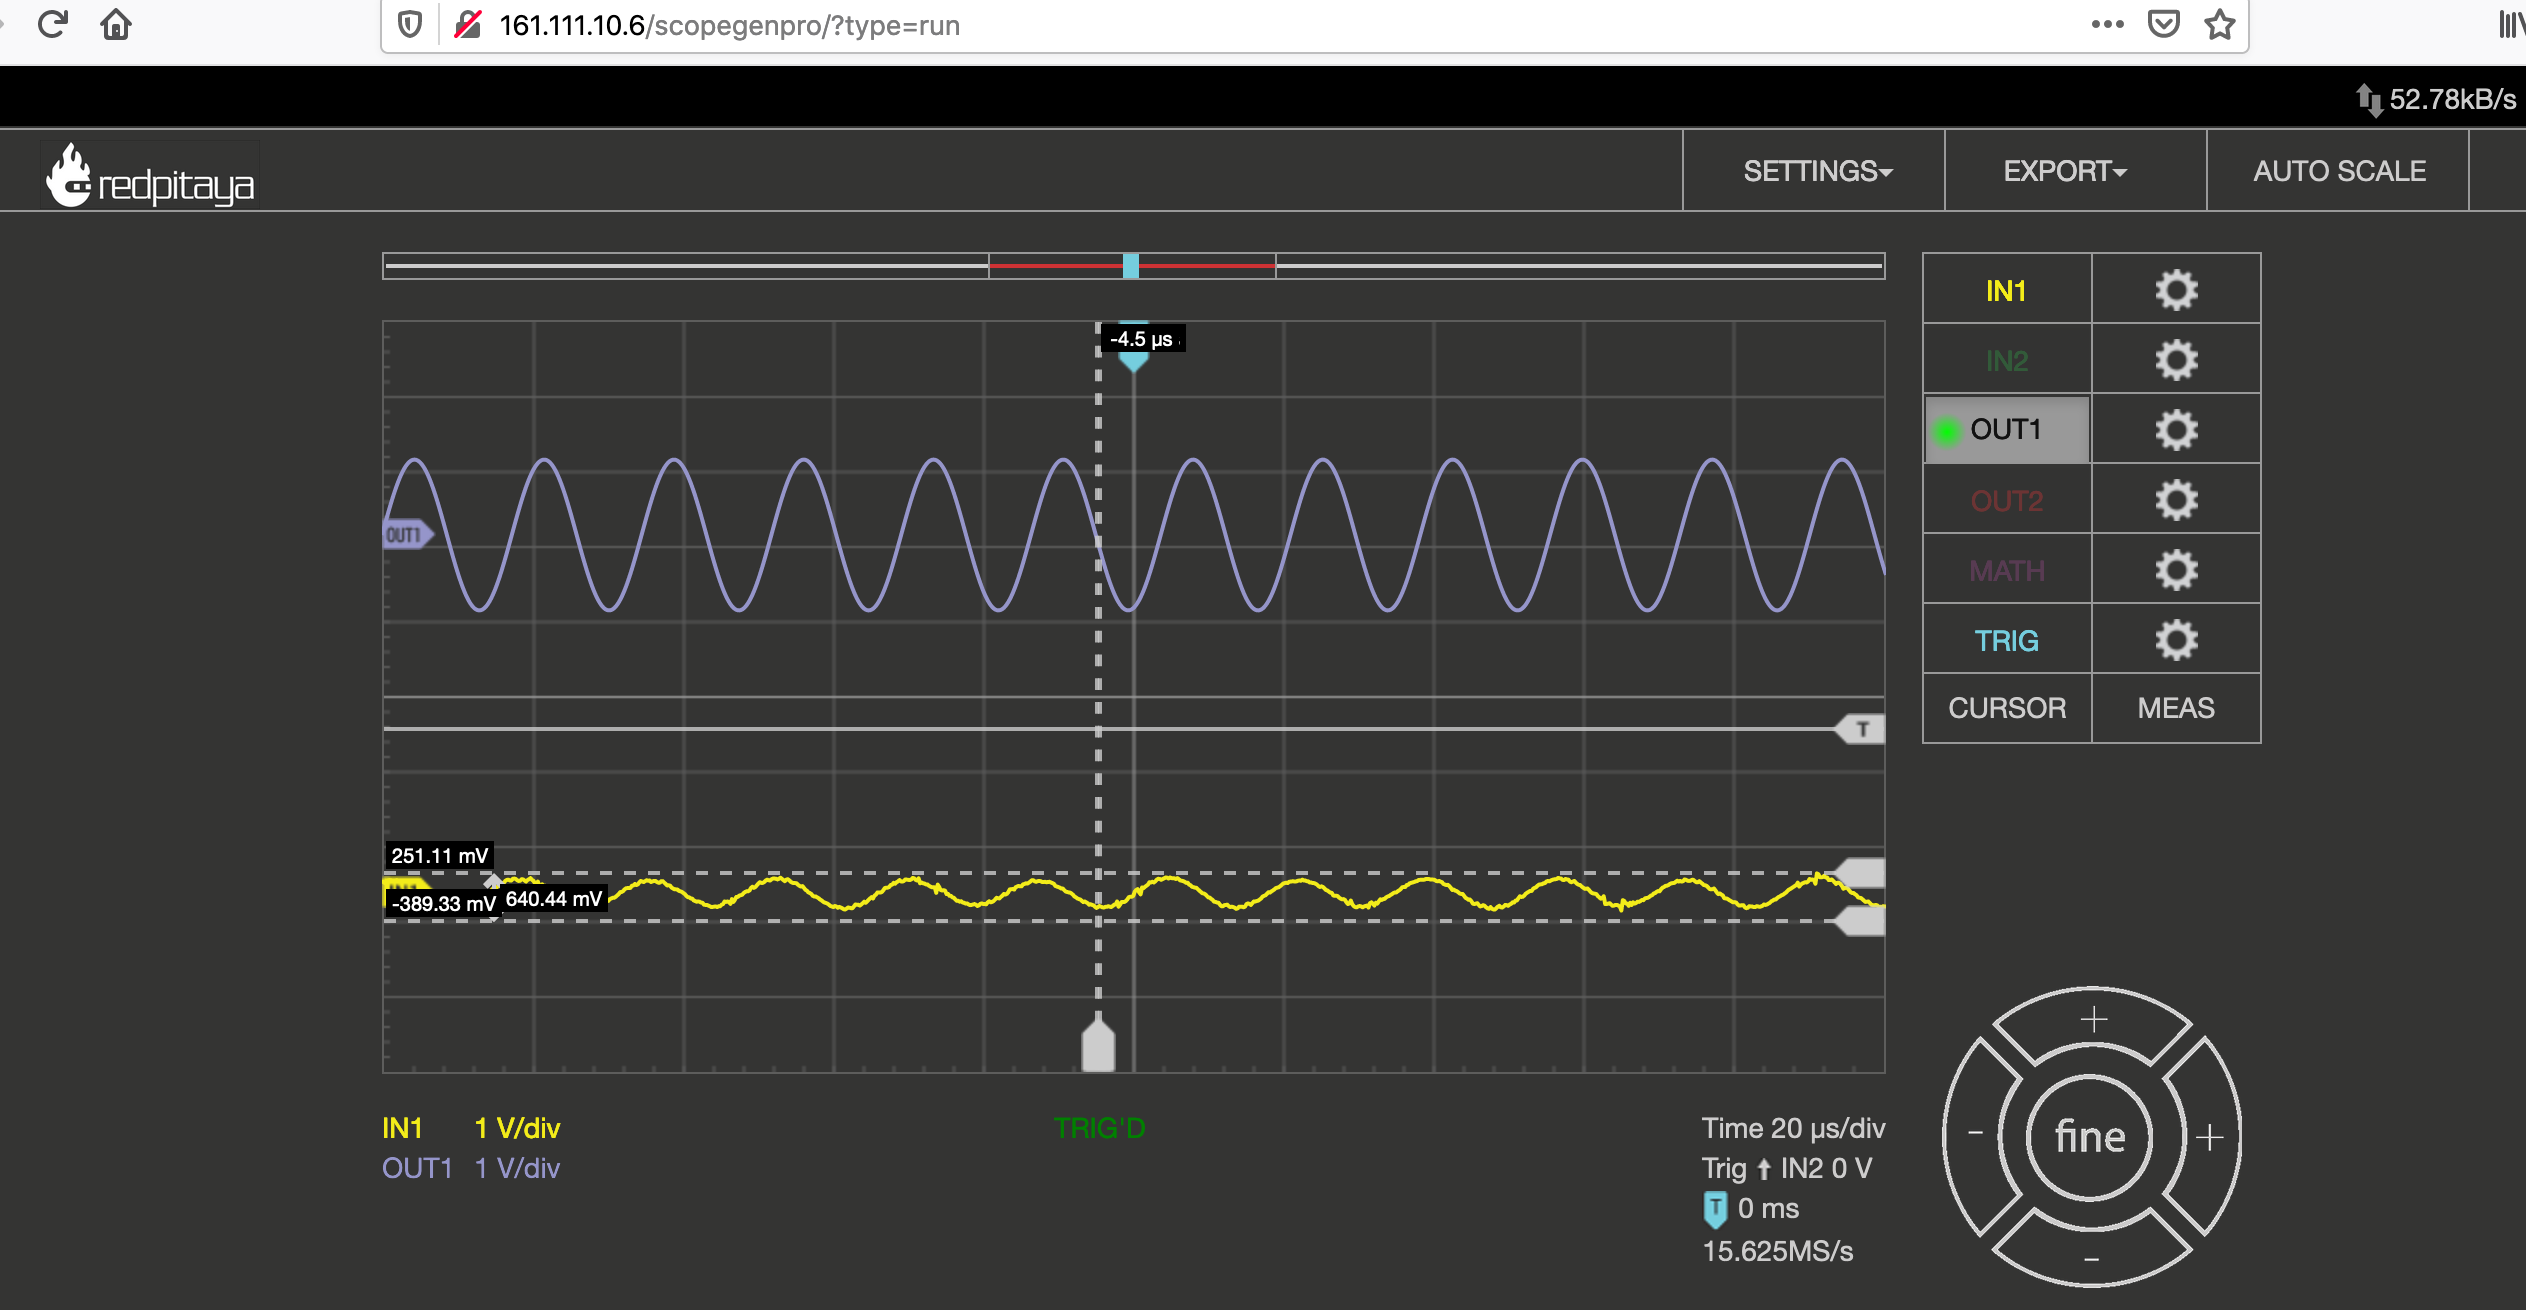
\includegraphics[width=0.8\textwidth]{images2/measurement2} 
		\caption{Generated (blue) and measured signal (yellow).}
		\label{fig:m2}
	\end{center}
\end{figure}


We have developed the data acquisition system based on the LabVIEW software \cite{labview}. The Figure \ref{fig:project} shows the project structured named ``coil measurements". Once we have closed the web browser, we need to generate a signal from the Red Pitaya board. By doing so, we run the file named ``signal generator"  in order to generate a signal.

\begin{figure}%[!h]
	\begin{center}
		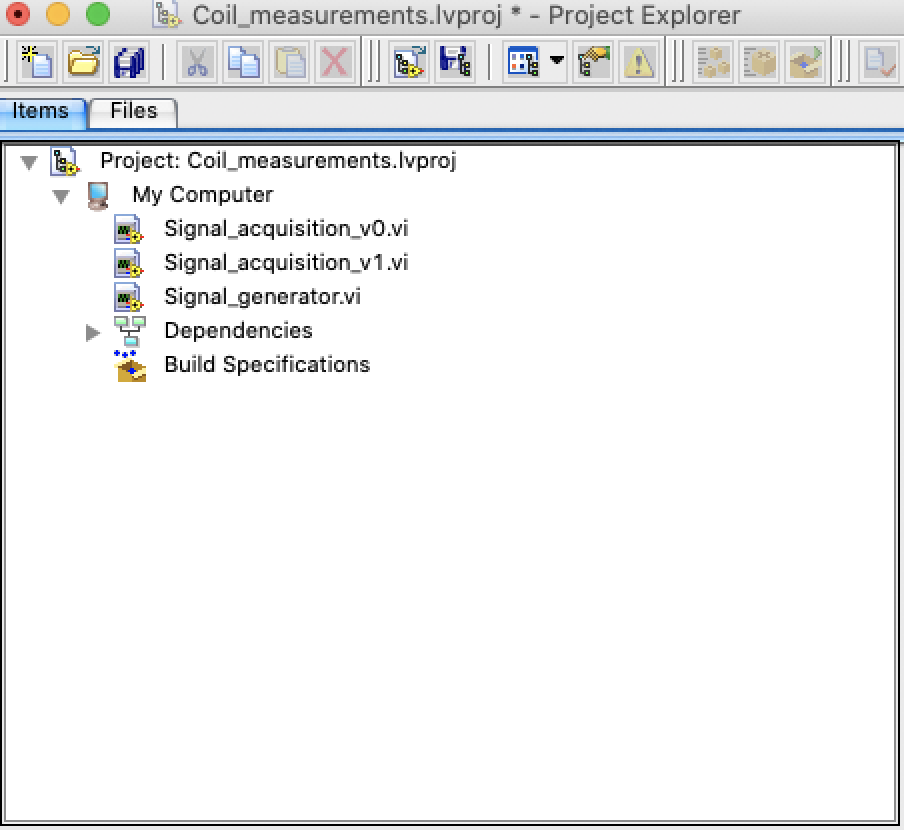
\includegraphics[width=0.25\textwidth]{images2/project} 
		\caption{LabVIEW project.}
		\label{fig:project}
	\end{center}
\end{figure}

We also open the file called ``signal acquisition v1"\footnote{We select the correct IP direction (i.e. 161.111.10.6). We recommend to check the error windows to be sure of the correct configuration. If TCP error connection appears, we need to be sure of IP configuration. Restart the Board and procedure all step from the scratch.}. Two graphs display the reference generated signal and the signal to be measured. Both signals are compared to obtain the amplitude value (Figure \ref{fig:labview1}). 


\begin{figure}[!h]
	\begin{center}
		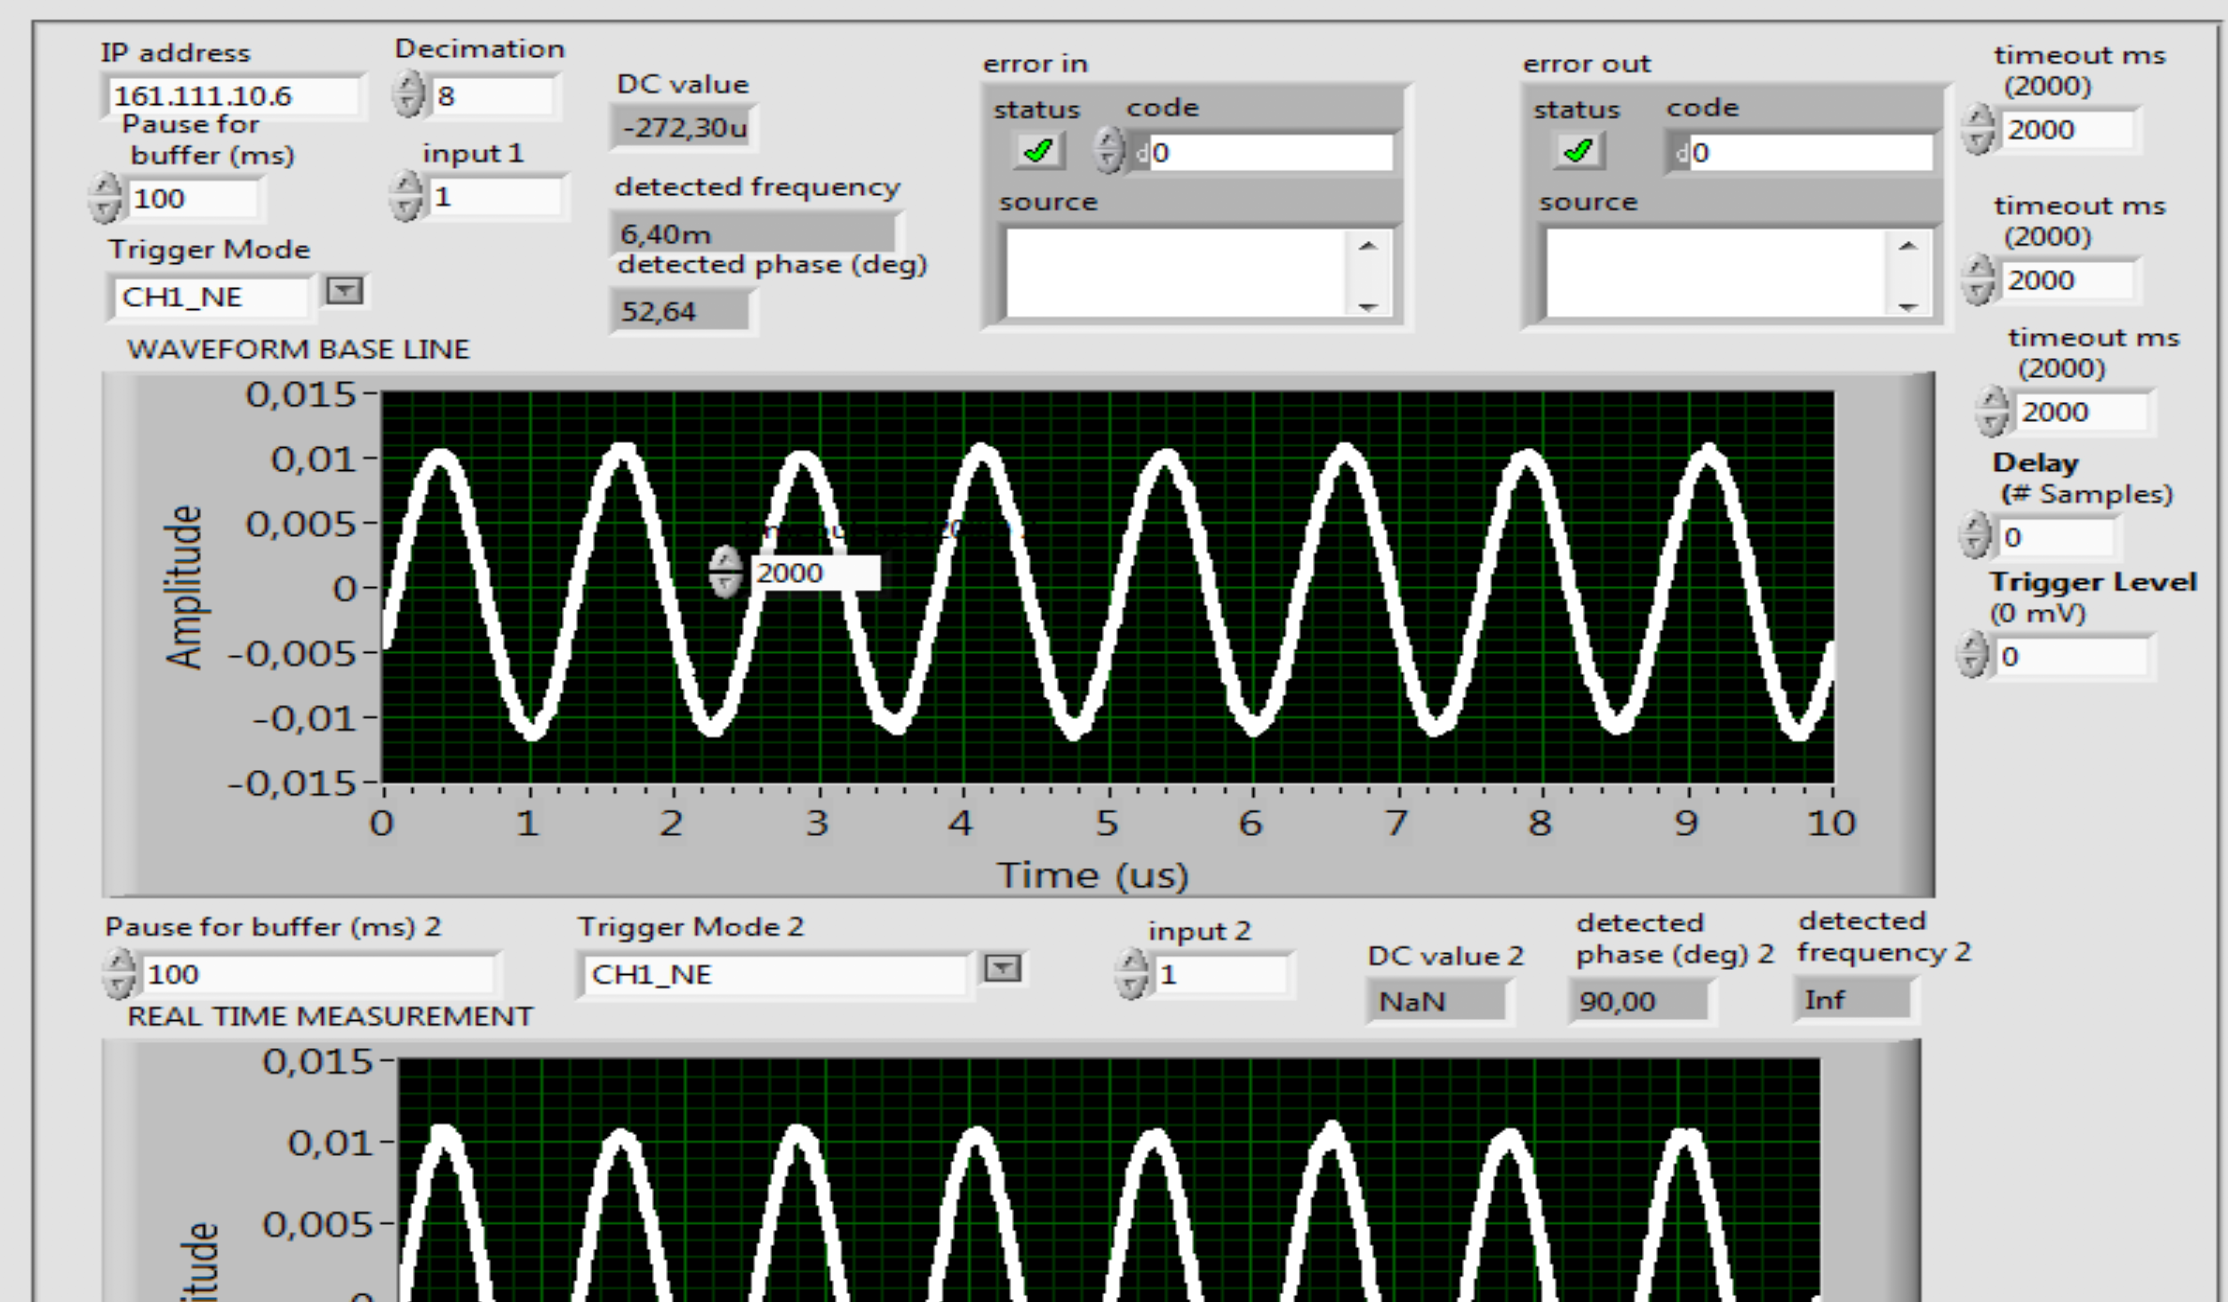
\includegraphics[width=0.7\textwidth]{images2/labview1} 
		\caption{LabVIEW software for the signal generator and the reference signal.}
		\label{fig:labview1}
	\end{center}
\end{figure}

The Figure \ref{fig:labview2} presents the results in terms of variation in amplitude and phase. First, we need to procedure the activation of the reference waveform base line.  Finally, we execute the amplitude measurement in order to obtain the amplitude result. \footnote{We have the possibility to save the results by activating the ``save" bottom.}

\begin{figure}[!h]
	\begin{center}
		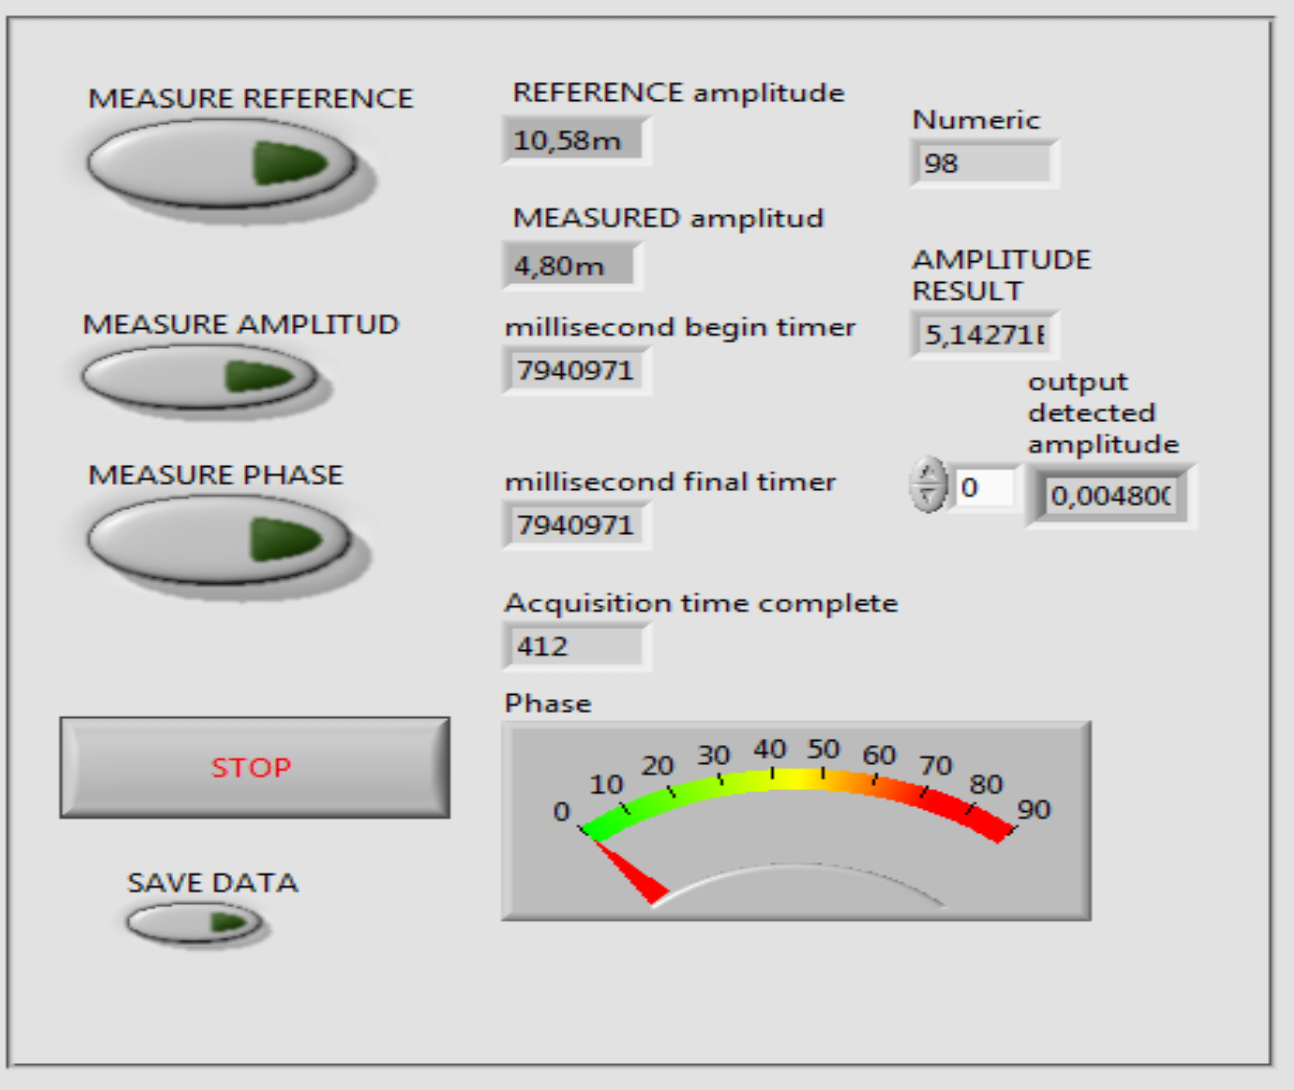
\includegraphics[width=0.7\textwidth]{images2/labview2} 
		\caption{LabVIEW software for the measurement results.}
		\label{fig:labview2}
	\end{center}
\end{figure}



We need to be sure to close TCP connection and we strongly recommend to stop the acquisition by pressing the ``STOP" bottom.  Sometimes, warning message up with the error 56, connection timeout. It is caused by LabVIEW code is not receiving a response from the network within a user-defined time limit. This error is a generic timeout error and can be the result of many different factors. Te following link explains how to solve the issue: \href{https://knowledge.ni.com/KnowledgeArticleDetails?id=kA00Z0000019Lz2SAE&l=es-ES}{Error 56 TCP Labview.}
If we open a connection to the board, we should use TCP Open. When opening connections to remote devices all we need is the TCP Open followed by the TCP Read/TCP Write and finally a TCP Close when communications are complete. 

The LabVIEW code and the manual is uploaded in the
\href{https://github.com/charlicruz/coil_measurements}{Github repository.}

%\begin{figure}%[!h]
%	\begin{center}
%		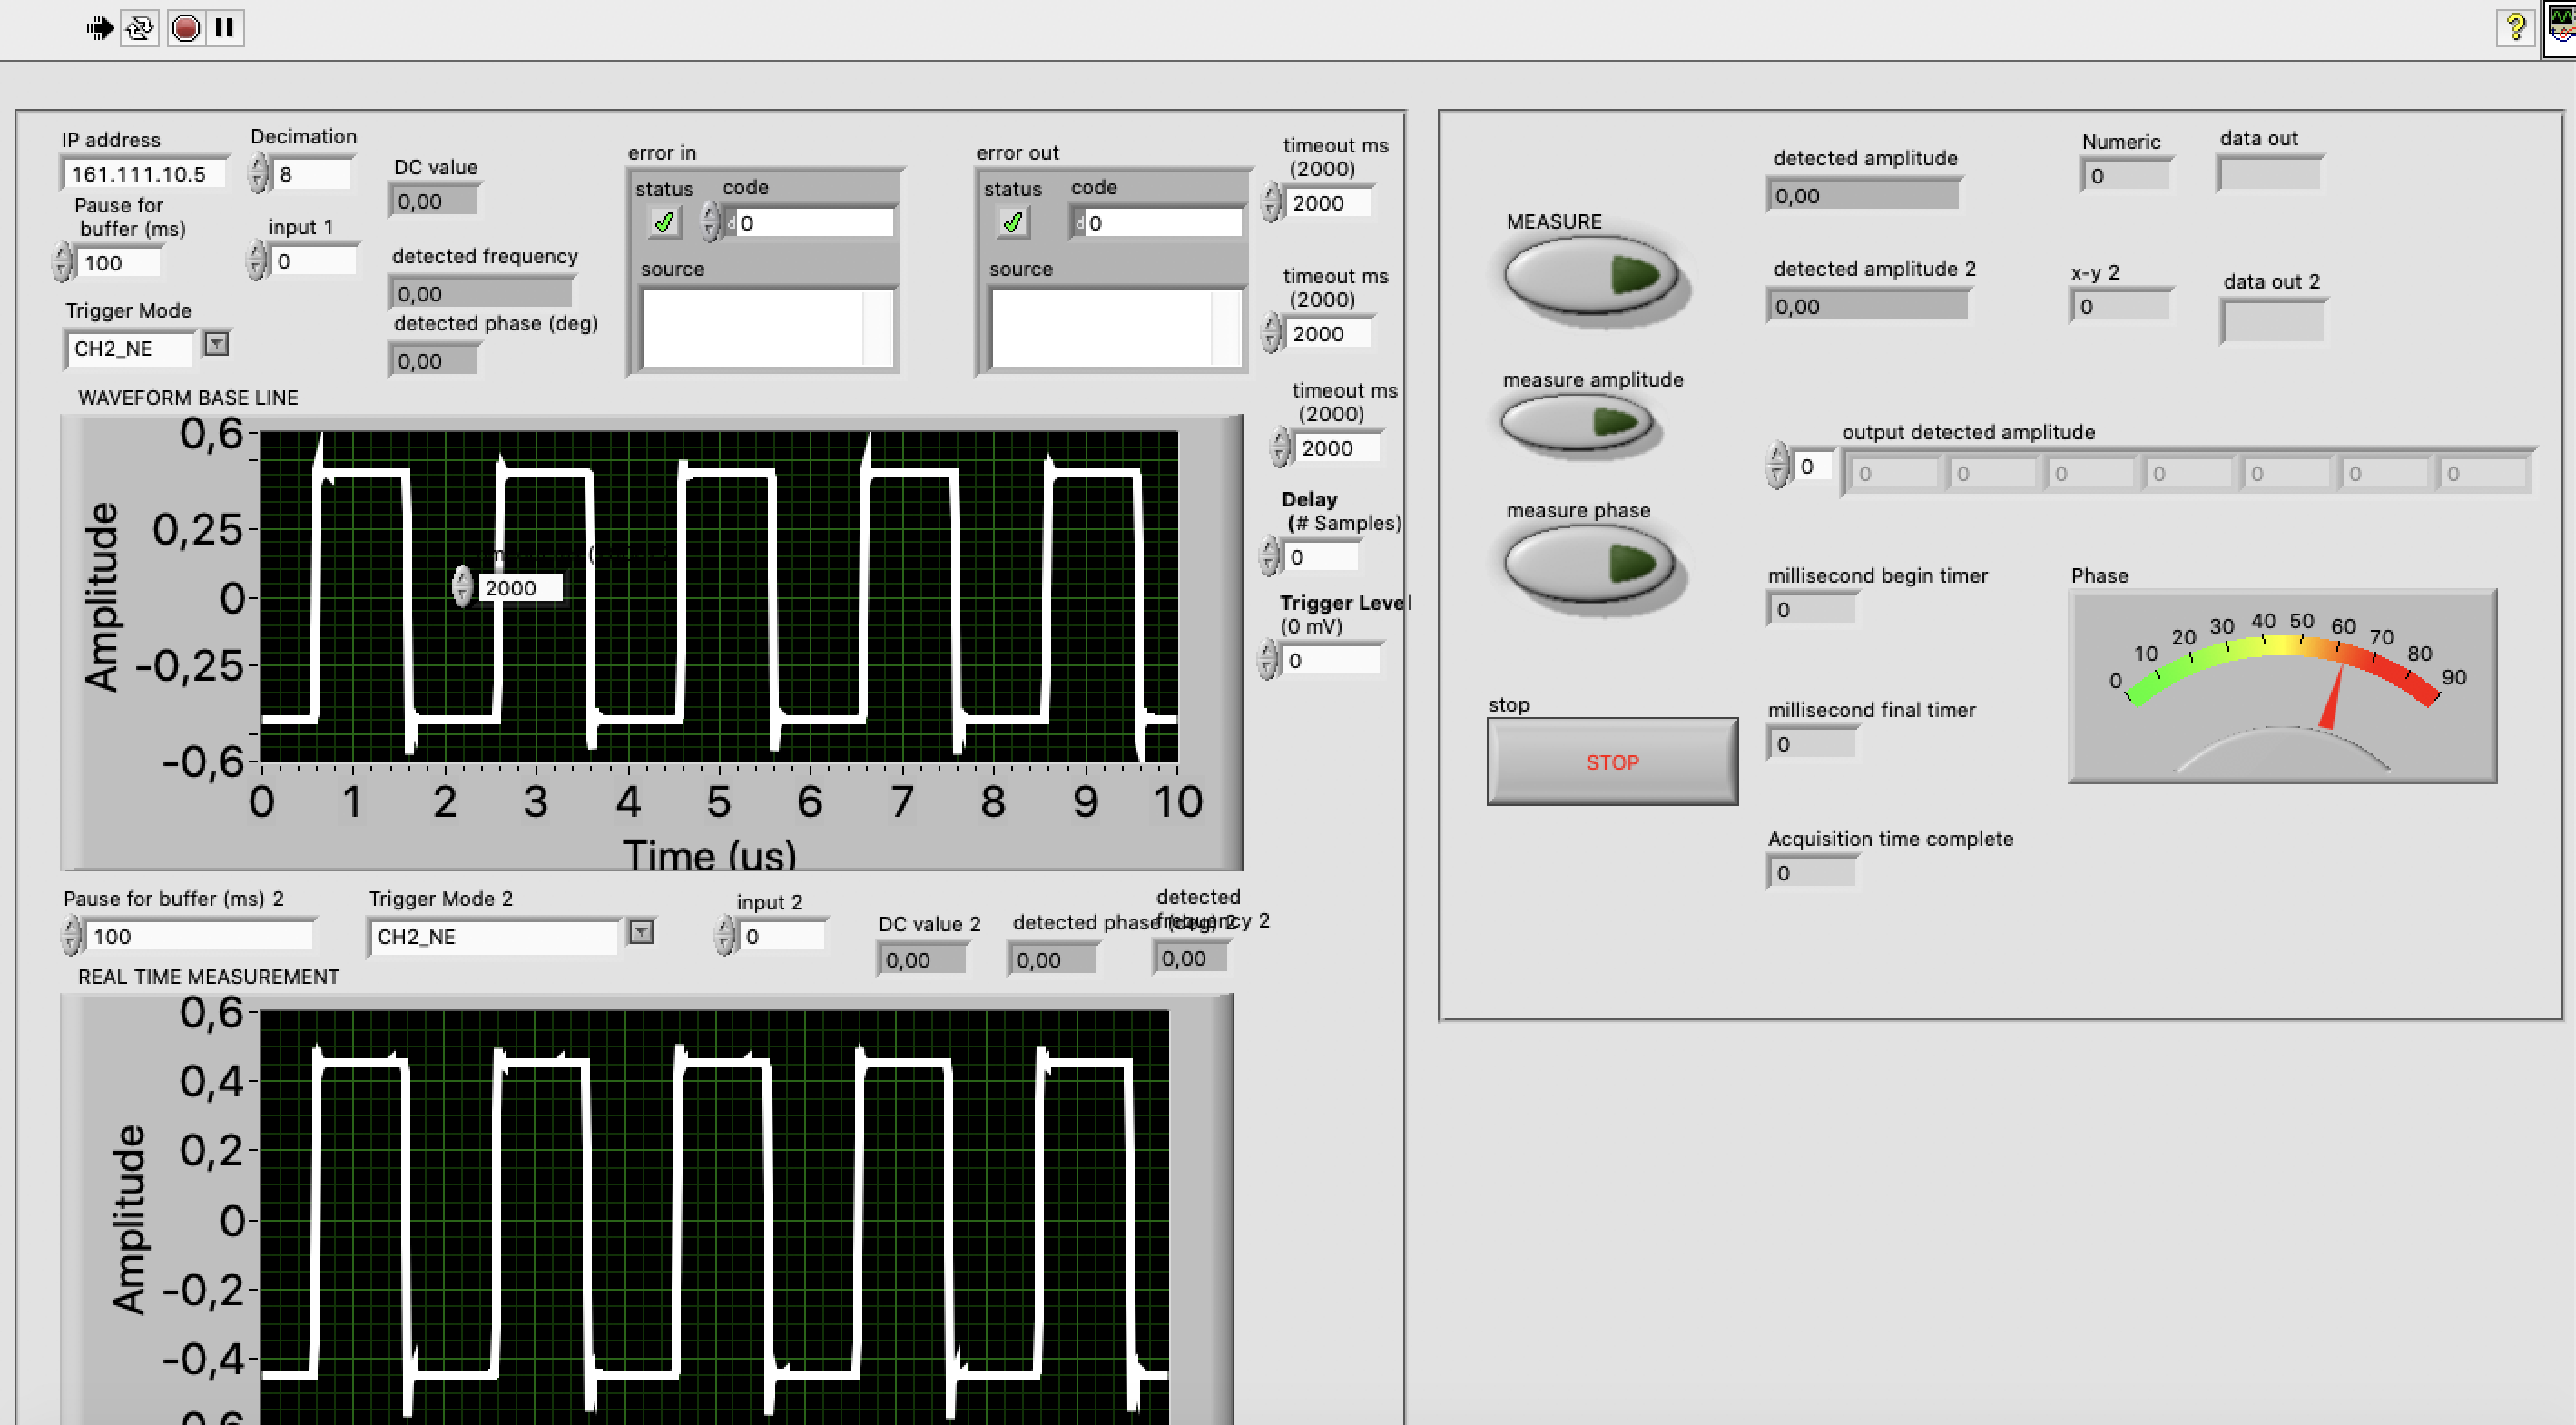
\includegraphics[width=0.6\textwidth]{images2/labview} 
%		\caption{LabVIEW software for data acquisition.}
%		\label{fig:labview}
%	\end{center}
%\end{figure}


\bibliographystyle{plain}
\bibliography{M335}

\end{document}
